\documentclass[a4paper,10pt, twoside]{report}
\usepackage[utf8]{inputenc}
\usepackage[T1]{fontenc}
\usepackage[french]{babel}

\usepackage{titlesec, blindtext, color}
\usepackage{setspace}
\usepackage{footnote}
\usepackage{etoolbox}

% \usepackage[left,modulo]{lineno}

\usepackage[export]{adjustbox}
\usepackage{array}
\usepackage{color, colortbl}
\usepackage{listings}
\usepackage{xcolor}

\usepackage{float}
\usepackage{fancyhdr}
\usepackage{fancyvrb}
\usepackage{graphicx}
\usepackage[top=2cm, bottom=2cm, left=2.5cm, right=2.5cm]{geometry}

\usepackage[hidelinks]{hyperref}

% page style
\pagestyle{fancy}
\setlength{\headheight}{49pt}
\setlength{\footskip}{42pt}
\setlength{\textheight}{0.93\textheight}

% header
\fancyhead[R]{
\includegraphics[width=5cm]{logo_sciences.png}}
\fancyhead[L]{
\includegraphics[width=5cm]{logo_arksens.png}}

% footer
\fancyfoot[C]{Rapport de stage --- Master 2 FSIL\\Ludovic Lubeigt}
\fancyfoot[RO, LE] {\thepage}

% colors
\definecolor{gray73}{gray}{0.73}
\definecolor{arkred}{rgb}{0.592, 0.145, 0.168}
\colorlet{punct}{red!60!black}
\definecolor{background}{HTML}{EEEEEE}
\definecolor{delim}{RGB}{20,105,176}
\colorlet{numb}{magenta!60!black}

% commands
\newcommand{\hsp}{\hspace{20pt}}
\titleformat{\chapter}[hang]{\Huge\bfseries}
{\thechapter\hsp\textcolor{gray73}{|}\hsp}{0pt}{\Huge\bfseries}
\titleformat*{\section}{\LARGE\bfseries}
\titleformat*{\subsection}{\Large\bfseries}
\titleformat{\subsubsection}{\large\bfseries}{}{}
{\refstepcounter{subsubsection}~\thesubsubsection~}
\titleformat{\paragraph}{\bfseries\itshape}{}{}{\\}

\patchcmd{\part}{\thispagestyle{plain}}{\thispagestyle{fancy}}
  {}{\errmessage{Cannot patch \string\part}}

\graphicspath{{../images/}}


\lstdefinelanguage{json}{
    basicstyle=\normalfont\ttfamily,
%     numbers=left,
    numberstyle=\scriptsize,
    stepnumber=1,
    numbersep=8pt,
    showstringspaces=false,
    breaklines=true,
    frame=single, % line
%     backgroundcolor=\color{background},
    literate=
     *{0}{{{\color{numb}0}}}{1}
      {1}{{{\color{numb}1}}}{1}
      {2}{{{\color{numb}2}}}{1}
      {3}{{{\color{numb}3}}}{1}
      {4}{{{\color{numb}4}}}{1}
      {5}{{{\color{numb}5}}}{1}
      {6}{{{\color{numb}6}}}{1}
      {7}{{{\color{numb}7}}}{1}
      {8}{{{\color{numb}8}}}{1}
      {9}{{{\color{numb}9}}}{1}
      {:}{{{\color{punct}{:}}}}{1}
      {,}{{{\color{punct}{,}}}}{1}
      {\{}{{{\color{delim}{\{}}}}{1}
      {\}}{{{\color{delim}{\}}}}}{1}
      {[}{{{\color{delim}{[}}}}{1}
      {]}{{{\color{delim}{]}}}}{1},
}

\setcounter{tocdepth}{2}

\begin{document}
\begin{spacing}{1.2}
 
% Page de garde
\begin{titlepage}
  \newgeometry{top=2cm, bottom=2cm, left=2cm, right=2cm}
  
  \begin{center}
    
\includegraphics[width=9cm]{logo_sciences.png}\\[2cm]
    
    \textsc{\bfseries\Large Rapport de stage\\[0.3cm]
    Master 2 -- Fiabilité, Sécurité et
    Intégration Logicielle\\[0.3cm]
        Parcours Fiabilité et Sécurité Informatique}\\[0.3cm]

    \rule{\linewidth}{1mm} \\[1cm]

    \textsc{\bfseries\huge Conception \&  développement système de backup
    chiffré et incrémental en C/C++}\\[1cm]

    \rule{\linewidth}{1mm}\\[1.5cm]

    \textsc{\huge Arksens Cyber Security}\\[2cm]
    
    \begin{figure}[H]
      \begin{minipage}[t]{8cm}
        \centering
        
\includegraphics[scale=0.50]{logo_adhara.png}
      \end{minipage}
      \begin{minipage}[t]{8cm}
        \centering
        
\includegraphics[width=7cm]{logo_arksens.png}
      \end{minipage}\\[1.3cm]
    \end{figure}
      
    \begin{minipage}{0.4\textwidth}
      \begin{flushleft} \large
        \emph{\bfseries Auteur :}\\
        Ludovic \textsc{Lubeigt}
      \end{flushleft}
    \end{minipage}
    \begin{minipage}{0.4\textwidth}
      \begin{flushright}
        \large \emph{\bfseries Tuteur Entreprise :}\\
        Gaëtan \textsc{van Diemen}\\[0.2cm]
        \emph{\bfseries Enseignant :}\\
        Jean-Luc \textsc{Massat}
      \end{flushright}
    \end{minipage}\\[1.5cm]
      
    \large\emph{\bfseries Année Universitaire :}\\
    2014 -- 2015

  \end{center}
\end{titlepage}

\begin{abstract}

Ce document présente le travail réalisé lors du stage de fin d'étude
à Arksens Ltd. à l'île Maurice entre le 1\up{er} avril 2015 et le 11
septembre 2015 dans le cadre du Master 2 Fiabilité et Sécurité
Informatique à l'Université d'Aix-Marseille.

Le rapport est découpé en deux parties. Une première servant de rapport
de synthèse et présentant l'entreprise, le sujet de stage, le
travail effectué de même que l'environnement de travail et les éventuelles
difficultés rencontrées.
La seconde partie apporte un aspect technique au rapport et permet de 
présenter le travail réalisé plus en détail.
\end{abstract}

\chapter*{Remerciements}
\thispagestyle{fancy}
Je tiens tout d'abord à remercier l'équipe pédagogique de la faculté des
sciences de l'université d'Aix-Marseille qui m'a permis d'avoir les
connaissances et les aptitudes nécessaires au bon déroulement de ce stage.

Je remercie également la société Arksens pour m'avoir permis de faire mon
stage chez eux. Tout particulièrement, je remercie David Terranova et Gaëtan
van Diemen qui m'ont accueilli à l'île Maurice et suivi au jour le jour
durant ces six mois, mais également Michaël Colaone et le reste de
l'équipe pour l'accueil et la bonne ambiance au sein de l'entreprise.

Enfin je remercie toutes les personnes que je peux oublier mais qui m'ont
aidé, dans l'écriture de ce rapport, dans le cadre du stage ou qui m'ont
tout simplement fait découvrir l'île Maurice.

Je tiens tout particulièrement à remercier Sir Daniel Brands of House Brands,
the first of His Name, King of the Dutch, King of the flatlands and the first
Men, Breaker of Cars and Father of the Bikers.

\clearpage
\pagestyle{fancy}
\tableofcontents
\clearpage

% \linenumbers
\part{Rapport}
\thispagestyle{empty}
\chapter{Introduction}
\thispagestyle{fancy}
Dans le cadre du Master professionnel \textit{Fiabilité, Sécurité et
Intégration logicielle}, parcours \textit{Fiabilité et Sécurité
Informatique} à l'\textit{Université d'Aix-Marseille}, un stage de fin
d'étude doit être effectué en entreprise pour valider les acquis et
rentrer dans le monde professionnel.

J'ai réalisé ce stage entre le 1\up{er} avril et le 11 septembre 2015, soit
une période de cinq mois et demi, dans l'entreprise \textit{Adhara Cyber
Security}, renommée \textit{Arksens} au 1\up{er} juillet.

Ce stage fut donc l'occasion pour moi de mettre en pratique mes connaissances,
acquises tout au long de mon parcours universitaire, dans un environnement
professionnel et de m'en servir pour mener au mieux la mission qui m'a
été confiée. Ma mission, durant ce stage, a été de concevoir et
dévélopper un système de backup incrémentale et sécurisé, offrant
une encryption en local des données des utilisateurs. J'ai ainsi procédé
à la rédaction du plan de développement puis à l'implémentation de
celui-ci, et j'ai ainsi participé au processus de création, jusqu'à un
stade avancé, de ce qui peut être qualifié de gros projet.

Ce rapport présente le déroulement du stage ainsi que le travail accompli
au sein de l'entreprise durant ces six mois.

\chapter{Présentation de l'entreprise}
\thispagestyle{fancy}
Créée en 2013 sous le nom d'\textit{Adhara Cyber Security} avant
d'être renommée \textit{Arksens} au 1\up{er} juillet 2015, l'entreprise 
dans laquelle j'ai effectué mon stage est spécialisée en sécurité
informatique. L'entreprise se développe sur trois continents grâce à une
approche novatrice et répondant aux besoins des entreprises et
administrations de toutes tailles.

Le changement de nom a fait suite à une évolution des clients puisque
l'entreprise, bien que principalement prestataire de service pour des PME
s'est ouverte aux entreprises de taille plus importante. Revoyant leur
stratégie de commercialisation et de communication, l'entreprise se devait
donc de changer de nom.

\section{Présence dans le monde}
Aujourd'hui \textit{Arksens} est donc présent dans trois pays chacun sur
un continent différent (voir figure~\ref{mapArksens}) offrant ainsi aux
utilisateurs un service de proximité :
\begin{itemize}
  \item Abu Dhabi aux Émirats Arabes Unis pour les activités au Moyen
  Orient.
  \item Pamplemousses à l’île Maurice pour les activités africaines.
  \item Paris en France pour les activités européennes.
\end{itemize}

\begin{figure}[h!]
  \centering
  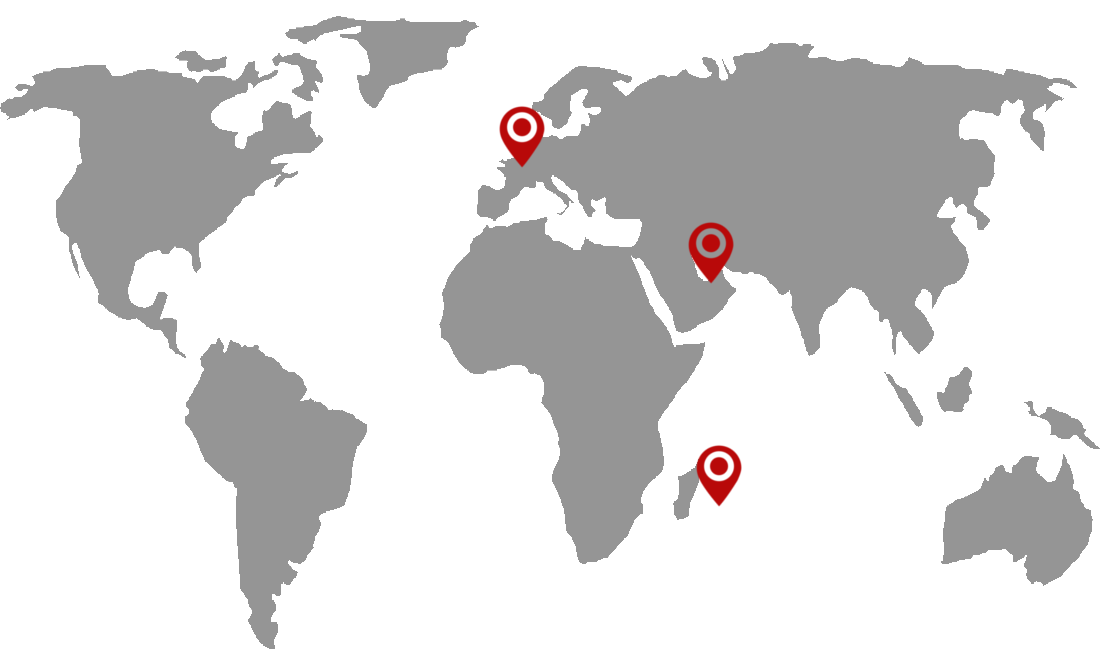
\includegraphics[scale=0.30]{map_arksens.png}
  \caption{\label{mapArksens} Où trouver Arksens}
\end{figure}
      
\section{Produits, solutions et offres}
\subsection{Les produits et solutions de sécurité}
\textit{Arksens} propose aux entreprises 6 produits et solutions autour de la
sécurité informatique. Une rapide description de ces produits se trouve
table~\ref{tabProduits} :
\begin{table}[h!]
  \centering
  \def\arraystretch{1.5}
  \setlength{\fboxsep}{13pt} % padding
  \setlength{\fboxrule}{0pt} % frame
  \begin{tabular}{m{6cm}m{6cm}}
   \rowcolor{arkred} 
    \arrayrulecolor{gray73}\hline
    \color{white} \textbf{Produit} & \color{white} \textbf{Description} \\
    
\includegraphics[width=5cm, fbox]{produits/mail.png} & Protéger l'information
    transitant par les mails. Hébergement de serveur email sécurisé dans
    un cloud dédié.\\
    \hline
    
\includegraphics[width=5cm, fbox]{produits/whisper.png} & Communications voix
    et images sécurisés et anonymes.\\
    \hline
    
\includegraphics[width=5cm, fbox]{produits/backup.png} & Système de
    chiffrement et de sauvegarde des données dans un cloud dédié.\\
    \hline
    
\includegraphics[width=5cm, fbox]{produits/gateway.png} & Sécuriser et
    rendre anonyme la navigation sur Internet.\\
    \hline
    
\includegraphics[width=5cm, fbox]{produits/endpoint.png} & Sécuriser les
    postes utilisateurs en locales. C'est une ligne de défense pour palier
    à la diffusion d'éventuels logiciels malveillants (virus, chevaux de
    Troie, vers, logiciels espions,\ldots{}) sur les ordinateurs et les
    serveurs.\\
    \hline
    
\includegraphics[width=5cm, fbox]{produits/nomad.png} & Sécuriser les
    données personnelles sur appareils mobiles.\\
    \hline
  \end{tabular}
  \caption{\label{tabProduits} Produits et solutions par \textit{Arksens}}
\end{table}

L'ensemble des produits et solutions proposés par l'entreprise sont décrit
de manière plus complète sur leur site web~\cite{refArksens}.

\subsection{Les offres de cloud}
L'entreprise propose également des offres autour du Cloud\footnote{
Exploitation de la puissance de calcul ou de stockage de serveurs distants
par l'intermédiaire d'un réseau, généralement l'Internet.}

\begin{itemize}
  \item Offre 1 - Pure cloud
  \noindent
  \begin{itemize}
    \item 100 \% des services sont hébergés
    \item La gestion est assurée par \textit{Arksens}
    \item Des fonctionnalités supplémentaires sont proposées telles que
    l'hébergement de fichiers ou de logiciels
  \end{itemize}
  \item Offre 2 - Hybrid cloud
  \noindent
  \begin{itemize}
    \item Un hébergement local avec une ``box'' chifrée et une
    réplication sur le cloud \textit{Arksens}
    \item La gestion est assurée par \textit{Arksens}
    \item Idéal pour les clients souhaitant une réplication dans leurs
    locaux
  \end{itemize}
  \item Offre 3 - Private cloud
  \noindent
  \begin{itemize}
    \item Le cloud est présent uniquement chez le client dans une salle de
    serveurs ou dans un centre de données
    \item La gestion est assurée par \textit{Arksens}
    \item Idéal pour les clients souhaitant stocker l'ensemble des services
    et des données localement (comme les banques, la défense,
    l'audit\ldots{})
  \end{itemize}
\end{itemize}

Avec 3 offres de cloud comportant l'ensemble des solutions de sécurité
cité précédemment, \textit{Arksens} peut répondre à l'ensemble des besoins
de ses clients actuels.

\section{L'idéologie de l'entreprise}
\subsection{La politique des centres de données}

Pour chaque service, \textit{Arksens} fournit le matériel (centres de
données), le produit et le support qui va avec. Pour être en mesure de
fournir les meilleurs services, elle possède une politique de sélection des
centres de données qu'elle utilise. Ci-dessous une liste représentant les
différents aspects les plus importants que doivent respecter les centres de
données :

\begin{itemize}
  \item Uniquement des Tier IV (Haute disponibilité\footnote{Mesure de
  performance. C'est le temps durant lequel le système est opérationnel par
  rapport à sa durée totale d'exploitation} : 99,995 \%)
  \item Toutes les données sont chiffrées sur les serveurs dédiés
  \item Les centres de données doivent se situés dans des pays libres
  respectant le \textit{Patriot Act}~\cite{refPatriotAct}
\end{itemize}

De ce fait l'entreprise a actuellement des centres de données en France
chez OVH~\cite{refOVH} qui lui confère en plus une solution contre les
attaques DDoS\footnote{Attaque par déni de service. Le principe est d'envoyer
une multitude de requête depuis plusieurs sources différentes pour rendre
un service indisponible.} et en Suisse chez AlpineDC~\cite{refAlpineDC} dont la
législation est une des plus restrictive en matière de protection de
données personnelles.

\subsection{La culture Open Source}

L'open source est une tradition dans l'entreprise. L'ensemble des
produits respectent les critères établis par l'Open Source
Initiative~\cite{refOSI}, à savoir :

\begin{itemize}
  \item Possibilité de redistribution
  \item Accès au code source
  \item Création de travaux déérivéés
\end{itemize}

Ce choix permet notamment d'accentuer la confiance avec les clients et
d'améliorer le niveau de sécurité des produits grâce aux avantages
suivants :

\begin{itemize}
  \item Logiciel indépendant : aucune porte dérobée
  (\textit{backdoor})\footnote{Fonctionnalité inconnue de l'utilisateur
  légitime et qui donne un accès secret au logiciel} ne peut
  être introduite par une organisation externe puisque les produits sont
  développés par \textit{Arksens} pour \textit{Arksens}
  \item Communauté : l'accès facile aux produits permet de créer une
  communauté d'utilisateurs capable sur le long terme de proposer un
  support sur les produit développés, des améliorations, mais aussi
  permet de déceler des bogues
  \item Code source accessible : tout le monde a accès au code source,
  rien n'est caché, la crédibilité et la qualité des produits est ainsi
  mise en avant
\end{itemize}

\section{Île Maurice}
L'île Maurice abrite les locaux accueillant le centre de recherche et
développement de l'entreprise. Les locaux se trouvent au Business Park de
Beau Plan (figure~\ref{beauPlan}) à Pamplemousses, ville située au
nord-ouest de l'île, à proximité de Port Louis. C'est donc là que
j'ai effectué mon stage.

\begin{figure}[h!]
  \centering
  \includegraphics[width=15cm]{beau_plan_soir.jpg}
  \caption{\label{beauPlan} Beau Plan Business Park}
\end{figure}

L'équipe a beaucoup évoluée entre mon arrivée et mon départ puisque
seulement trois personnes en plus du PDG, Michaël Colaone, étaient
présentes au 1\up{er} avril, date de début du stage : David Terranova,
directeur des opérations, Gaëtan van Diemen, chef de projet ainsi que
Daniel Brands, développeur web arrivé quelques jours auparavant.

L'équipe s'est agrandie par deux fois. D'abord à la mi-avril avec
l'arrivée de deux autres stagiaire, Didier Mannone et
Yves Colin de Verdière, puis au 1\up{er} mai avec l'arrivée d'Aymeric
Tabourin, ingénieur sécurité.

À mon départ, une restructuration était en cours et plusieurs changements
allait être apportés au niveau de l'équipe en place avec notamment le
départ de certains collaborateurs (licenciement, démission ou tout
simplement fin de stage). Ceci a précipité la fin de mon stage d'une
quinzaine de jour puisque j'ai arrêté celui-ci au 11 septembre bien qu'il
était initialement prévu de finir le 25 septembre.

Ces changements montrent que la vie d'une startup peut rapidement évoluer,
que ce soit dans un sens ou dans l'autre. En l'espace de six mois seulement
une période de recrutement s'en était donc suivi d'une restructuration
importante impliquant le départ de plusieurs employés.

Durant mon stage dans l'entreprise, la présence de collaborateurs
Néerlandais et Mauriciens a permis la création d'un environnement
international, bien que fortement francophone. Afin de pouvoir communiquer avec
l'ensemble des personnes de l'équipe, l'utilisation de l'anglais au quotidien
était donc une nécessité.

L'intégration dans l'équipe s'est donc faite assez facilement et rapidement
et c'est ainsi dans une ambiance généralement bonne, bien que quelque peu
compliquée sur la fin dû à la restructuration de l'entreprise s'est
déroulé ce stage de fin d'étude.

\chapter{Sujet de stage}
\thispagestyle{fancy}
\section{Contexte}
L'entreprise étant encore jeune et de petite taille, plusieurs des services
existant étaient basé sur des produits open source qui avaient été
intégré au \textit{manager} (voir figure~\ref{managerFront}).

Ce \textit{manager} est un environnement web développé et maintenu par
\textit{Arksens}. Il permet aux utilisateurs de gérer les services auxquels
ils ont souscrit à partir d'un unique endroit, centralisé, et ainsi
faciliter l'utilisation de ces derniers.

\begin{figure}[h!]
  \centering
  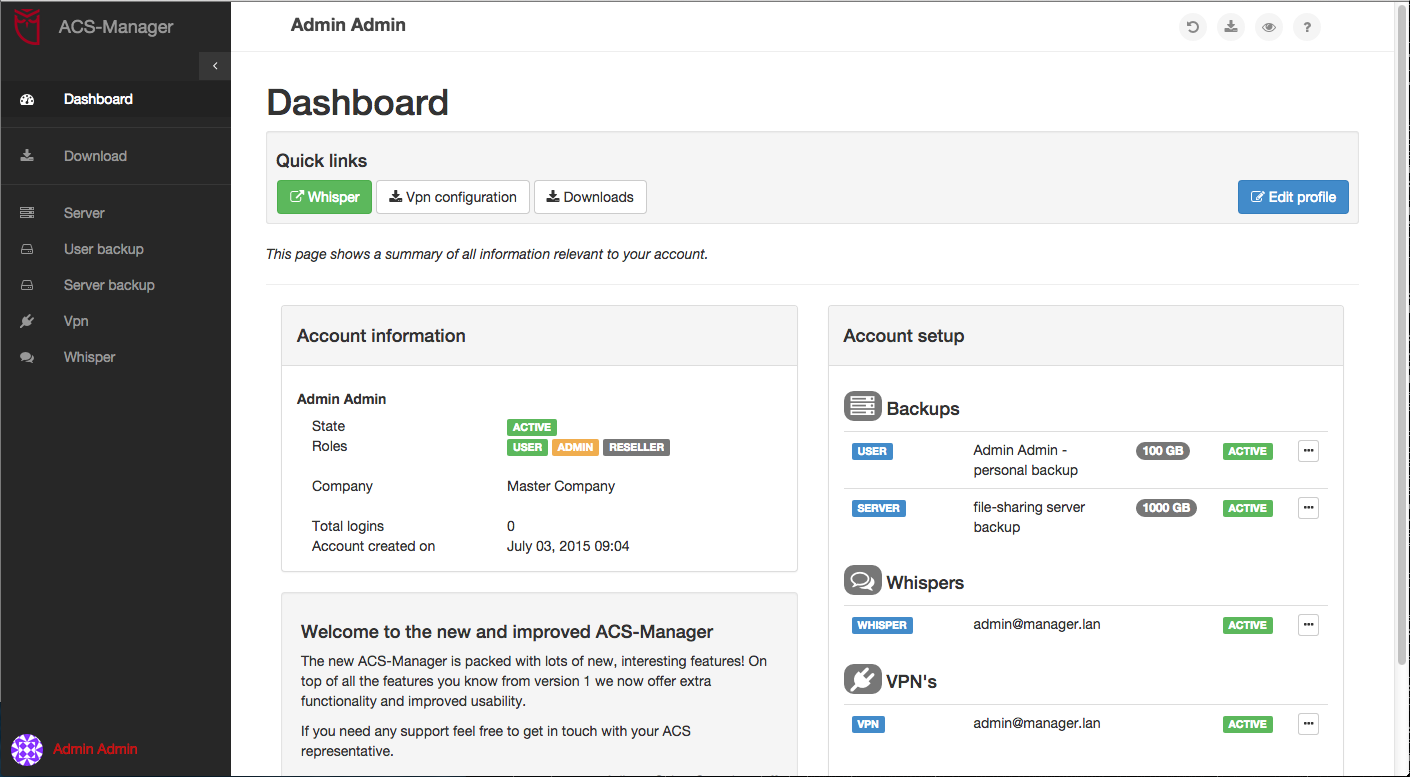
\includegraphics[width=15cm]{produits/manager.png}
  \caption{\label{managerFront} Page d'accueil du \textit{manager}}
\end{figure}

L'objectif de ce recrutement important était pour l'entreprise de petit à
petit développer ses propre solutions afin de proposer aux utilisateurs des
produits adaptés et répondant à leurs besoins tout en minimisant
l'utilisation de logiciels tiers.

De plus les systèmes de backup ne sont souvent pas considérés par les
entreprises avant qu'une perte de données, plus ou moins importante,
ne survienne. Conséquences financières, temps passé à reconstituer le
savoir évaporé ou encore impact sur la réputation de l'entreprise ne sont
que des exemples de ce qui peut arriver dans une telle situation. Pour
prévenir ce problème un système de backup est non seulement nécessaire
mais presque obligatoire.

Pour cela, \textit{Arksens} voulait offrir à ses clients un système de
sauvegarde fiable, sécurisé et optimisé afin de pouvoir être
exécuté sur les ordinateurs les moins performants. De plus la prise en
compte de connexions Internet pouvant être parfois très lentes était une
obligation. En particulier, une partie du marché visé par \textit{Arksens}
se trouve en Afrique où l'accès à un Internet rapide n'est pas toujours
aussi facile que ce qu'il peut y avoir en Europe.

C'est donc dans ce cadre que je suis arrivé et qu'il m'a été demandé
de créer la prochaine génération de backup pour \textit{Arksens}.

\section{Le sujet}
Ma mission pour ce stage était donc de faire la conception et le
développement d'un système de backup incrémental et dont les données
sauvegardées sont chiffrées en local, sur la machine client, avant d'être
envoyées sur des serveurs distant. Il me fallait donc développer un
client/serveur multi-plate-forme, robuste et sécurisé répondant à
la problématique suivante : combiner le chiffrement local avec la sauvegarde
incrémentale.

De plus le programme devra être \textit{multi-threadé} pour pouvoir
optimiser la sauvegarde des données. Entre autre, cela permettra de chiffrer
des blocs, constituant les fichiers, tout en envoyant au serveur ceux déjà
chiffrés.

Par ailleurs, allant être un service proposé aux entreprises, il doit être
pris en compte qu'un administrateur puisse gérer les différentes
sauvegardes ou être informé si un problème survient sur le poste d'un
employé lors de l'utilisation du logiciel.

Enfin, un système de quota devra être mis en place. Ce système permettant
aux entreprises de demander un plus ou moins grand quota selon la quantité de
données à sauvegarder. Celle-ci pouvant varier selon la taille ou la
fonction de l'entreprise, un quota permet une certaine flexibilité.

Ce backup permettrait donc, au premier lancement, de sauvegarder l'ensemble
d'un ou plusieurs dossier. À partir de la seconde sauvegarde, il ne faudrait
néanmoins sauvegarder que les changements sur les fichiers.

À mon arrivée, David et Gaëtan avait déjà des idées sur la
manière de réaliser ce système de sauvegarde, idées que nous verrons
plus loin dans ce rapport. Et c'est à partir de celles-ci que j'ai pu
démarrer mon travail, qui sera alors divisé en trois grandes phases :

\begin{itemize}
 \item Phase de documentation et de réflexions sur la problématique
 \item Conception logicielle
 \item Développement
\end{itemize}

La première phase de documentation et de réflexions consistait à
rechercher différentes solutions déjà existantes et potentiellement
exploitable avant de procéder à toute phase de conception.

La conception s'est faite en prenant en compte les contraintes existantes
et en se basant sur un travail de réflexions déjà effectué par David et
Gaëtan avant mon arrivée.

Enfin, en ce qui concerne le développement, une des contraintes que j'avais
était d'utiliser le C++ et de développer de manière orienté objet tout
en faisant en sorte que le code puisse être robuste, lisible, testable, et
donc facilement maintenable. De plus les librairies et \textit{framework}
utilisés devaient être sous licence libre afin d'être en droit de publier
l'ouvrage sous licence libre. Une dernière contrainte, mais pas des moindres,
était de développer en logiciel pour qu'il puisse tourner sur les
plate-formes répandues : \textit{Mac OSX}, \textit{Windows} et
\textit{GNU/Linux}.

Pour mener cette mission à bien, il avait été décidé qu'une réunion
hebdomadaire devait être réalisée afin que David et Gaëtan puissent
suivre l'avancement du projet mais aussi pour voir le travail effectué la
semaine précédente, essayer de résoudre tout problème qui aurait pu
survenir et planifier la semaine suivante.
C'est en tout cas dans cette optique là que nous avions commencé. Dans les
fait, le retour des clients de l'entreprise lors de mises à jour des produits
ou des réunions avec de potentiels futurs clients pouvaient prendre la
priorité et ainsi retarder ou annuler les réunions hebdomadaire.

\chapter{Déroulement du stage}
\thispagestyle{fancy}
Avant de commencer le projet en lui-même, David et Gaëtan m'ont fait part
de leur réflexion sur le possible fonctionnement du système de sauvegarde.

\begin{figure}[h!]
    \hspace{-4.5em}
    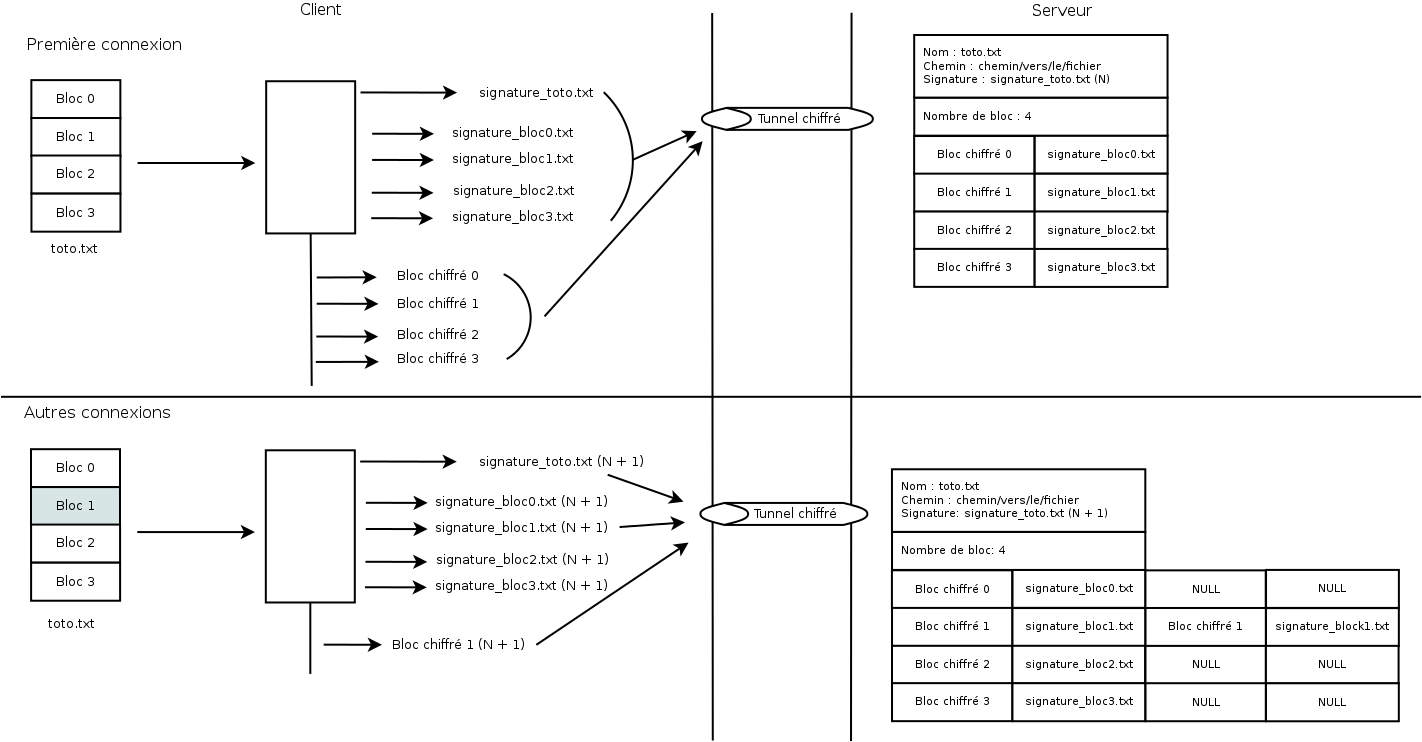
\includegraphics[width=19cm]{algo/schemaInitial.png}
    \caption{\label{schemaInitial} Schéma initial du fonctionnement du backup}
\end{figure}

Le système a deux comportement différent lors de la sauvegarde d'un fichier.
D'abord pour la première connexion, où une sauvegarde intégrale est
nécessaire, puis lors des connexions suivantes où seulement les
modifications doivent être envoyées.

Dans le premier cas, le fichier est découpé en blocs de taille égale
avant d'être chiffré puis envoyé accompagné des signatures calculés
pour chaque bloc ainsi que pour le fichier en lui même. Les signatures
permettant de vérifier l'intégrité des fichiers.

Le second cas est un peu plus complexe et décrit comme suit :
\begin{itemize}
 \item Calculer \textit{signature\_toto.txt} (\(N + 1\))
 \item Téléchager \textit{signature\_toto.txt} (\(N\))
 \item Comparer les deux signatures : si elles ne sont pas différentes, les
 fichiers n'ont pas à être comparé et on peut passer au fichier suivant
 sinon on continue
 \item Découper toto en bloc
 \item Calculer la signature de chaque bloc (\(N + 1\))
 \item Télécharger la signature de chaque bloc (\(N\))
 \item Comparer chaque signatures entre elles
 \item Pour chaque signature différente, envoyer sur le serveur le bloc
 chiffré correspondant accompagné de sa signature (\(N + 1\))
\end{itemize}

Dans le cas de la figure~\ref{schemaInitial}, le bloc 1 étant modifié, sa
signature, à \(N + 1\), ne correspond pas à la signature précédemment
calculée (\(N\)). Le bloc est donc chiffré avant d'être envoyé sur le
serveur avec sa signature \textit{signature\_bloc1.txt}.

\subparagraph{}
L'idée, bien qu'intéressante dans un premier temps, ne peut être
appliquée que dans un cas très particulier de fonctionnement et ne peut
donc pas être utilisé en tant que tel :
\begin{itemize}
 \item Si les modifications n'affecte pas la taille d'un bloc et que l'ordre
 des blocs est resté inchangé
\end{itemize}

Pour tout les autres cas (ajout, suppression, déplacement de tout ou partie
d'un bloc, etc.), l'algorithme ne pourrait pas fonctionner. Pour palier à
cela, j'ai donc dû imaginer un algorithme répondant à la problématique
et fonctionnant dans tout les cas imaginables.

\section{Travail de recherche}
\label{secTravailRecherche}
\subsection{Documentation}
Mon travail de recherche s'est fait à partir d'une liste de mots-clés qui
m'a été donné afin que l'on parle tous le même langage. Entre autre,
certaines définitions liées au backup et au chiffrement :
\begin{itemize}
 \item Backup incrémental\footnote{Sauvegarde de fichiers dont le principe est
 d'envoyer uniquement les fichiers modifiés depuis la dernière sauvegarde
 effectuée}
 \item Backup différentiel\footnote{Sauvegarde de fichiers dont le principe
 est d'envoyer uniquement les fichiers modifiés depuis la dernière
 sauvegarde complète effectuée}
 \item Transchiffrement\footnote{Technique consistant, lors d'un changement
 de clé de chiffrement, à déchiffrer l'ensemble des données avec la
 précédente clé puis à les re-chiffrer avec la nouvelle}
\end{itemize}

Mais aussi des logiciels déjà existant, de backup ou de synchronisation de
fichiers et à partir desquels il pouvait être intéressant de s'inspirer :
\begin{itemize}
 \item Syncthing~\cite{refSyncthing}
 \item rsync~\cite{refRsync}
\end{itemize}

\subsubsection{Syncthing}
\textit{Syncthing} est un logiciel permettant la synchronisation des données
entre plusieurs appareils au travers d'une communication sécurisée via TLS.
Les données n'étant jamais stockées sur un serveur tiers, uniquement les
différents ordinateurs utilisés y ont donc accès.

L'aspect intéressant de \textit{Syncthing} est pour nous le protocole de
communication, qui a été crée à l'occasion : Block Exchange Protocol
(BEP)~\cite{refBEP}. Ce protocole sous Creative Commons~\cite{refCC4.0}, est
donc une bonne source d'inspiration afin de faire la liaison entre notre client
et notre serveur.

\subsubsection{rsync}
\textit{rsync} est un programme de transfert de fichiers pour les systèmes
Unix. Le c\oe ur du programme est son algorithme schématisé
figure~\ref{rsyncAlgo} :
\textit{\flqq rsync algorithm \frqq}~\cite{refRsyncAlgo}.

\begin{figure}[h!]
    \centering
    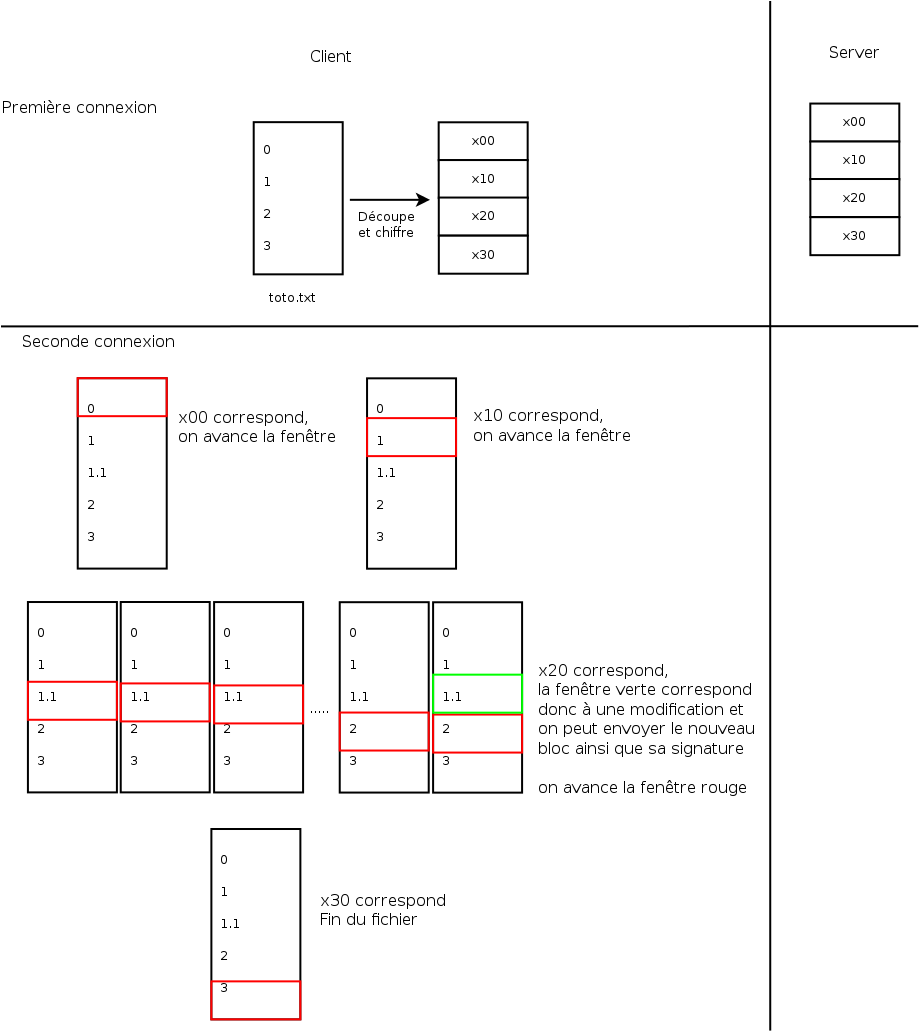
\includegraphics[width=15cm]{algo/rsyncalgo.png}
    \caption{\label{rsyncAlgo} Schéma montrant brièvement
    l'algorithme \textit{rsync}}
\end{figure}

Celui-ci va découper un fichier en plusieurs blocs de taille identique avant
de calculer, pour chacun, un \texttt{checksum} ainsi qu'un \texttt{hash}.

Pour n'envoyer que les parties modifiées d'un ficher, l'algorithme va créer
une fenêtre de la taille des blocs. Celle-ci va parcourir l'intégralité
du fichier octet par octet.

Pour chaque position de la fenêtre, le \texttt{checksum} --- rapide à
calculer mais dont le risque de collision est élevé --- est calculé et
comparé au \texttt{checksum} déjà calculé au précédent backup de
chaque bloc composant le fichier. Si un \textit{checksum} correspond, le
\texttt{hash} --- plus lent à calculer mais ayant un risque de collision
beaucoup plus faible, selon l'algorithme utilisé --- du bloc correspondant
est alors comparé. Si celui-ci est identique, la fenêtre correspond à un
bloc non modifié du fichier.

Ainsi, tout ce qui précède la fenêtre, et jusqu'au précédent bloc
trouvé, correspondant à une partie du fichier modifiée
(ajout/modification/suppression) et doit donc être synchronisé.

C'est en grande partie cet algorithme qui m'a permis d'en trouver un me
permettant de répondre à ma problématique. Problématique à la fois
similaire au problème de \textit{rsync} puisqu'il fallait comparer deux
fichiers distants pour n'envoyer que les changements mais également
différent dans la mesure où il n'est pas possible dans mon cas de maintenir
une liste de bloc de même taille au delà de la première sauvegarde.

\subsection{Réflexions}
Une fois cette phase de documentation réalisée, il était temps de trouver
un algorithme permettant d'identifier les parties d'un fichier ayant été
modifié depuis le précédent backup. Pour ce faire, et comme indiqué
dans la partie documentation, je me suis basé sur l'algorithme \textit{rsync}
pour, petit à petit, créer un algorithme qui permettait de répondre à ma
problématique.

\subsubsection{Chiffrement homomorphe}
Dans un premier temps, j'ai étudié la question de l'homomorphisme. Ce type
de chiffrement permet de réaliser des opérations sur des fichiers chiffrés
et de retourner le résultat chiffré. Ceci permet de faire des opérations
sans avoir à connaître le contenu d'un fichier.

\begin{itemize}
 \item \textbf{Fonctionnement :} Dans notre cas, il nous aurait permis de
 concatener sur le serveur l'ensemble des morceaux d'un fichier avant de le
 re-découper en bloc de taille égale puis de calculer pour chacun le
 \texttt{checksum} ainsi que le \texttt{hash}. Ceci aurait permis d'utiliser
 directement l'algorithme \textit{rsync} pour identifier les modifications
 faites sur un fichier.

 \item \textbf{Avantage :} Consommation de ressource et temps de calcul
 réduit sur la machine client.
 
 \item \textbf{Inconvénient :} En utilisant le chiffrement homomorphe, le
 plus gros du calcul se fait sur le serveur entre deux backup, et ceux pour
 chaque fichier de chaque utilisateur. Ce type de chiffrement est donc très
 demandeur de ressource du côté du serveur pour que le programme fonctionne
 correctement.

 \item \textbf{Problème :} Le chiffrement homomorphe est un domaine de
 recherche très prometteur mais pas encore assez avancé pour pouvoir
 être utilisé en production. De plus le temps de calcul est extrêmement
 élevé. Cette solution ne peut donc pas être utilisée aujourd'hui mais
 pourra peut-être un jour être envisagée dans une prochaine version du
backup.
\end{itemize}

\subsubsection{rsync revisité}
Étant donné que les fichiers doivent être chiffrés et déchiffrés
uniquement sur la machine hôte (le client), nous ne pouvons effectuer
d'opérations sur ceux-ci du serveur. Il fallait trouver un algorithme qui
permette de d'analyser un fichier en un temps fini. J'ai donc décidé de
baser mon travail sur le principe de fenêtre glissante utilisée pour
\textit{rsync}. Ne pouvant pas avoir des morceaux de fichier de taille
identique, il a fallu modifier l'algorithme pour prendre ceci en compte. Ainsi
avoir une fenêtre dynamique semblait être l'option à prendre.

\begin{itemize}
 \item \textbf{Fonctionnement :} L'algorithme utilise une fenêtre dynamique,
 parcourant l'intégralité du fichier et adaptant sa taille en fonction
 des longueurs des morceaux de fichier que nous avons.
 
 \item \textbf{Avantage :} Fait côté client, il n'y a pas une
 sur-utilisation des ressources serveurs qui est alors utilisé uniquement
 pour stocker les données une fois chiffrées.
 
 \item \textbf{Inconvénient :} Temps de calcul potentiellement grand,
 dépendant de la taille des fichiers à analyser ainsi que de ressources
 disponible sur la machine client.
\end{itemize}

C'est donc sur cette base que j'ai commencé l'étape suivante. Étape 
consistant à écrire un prototype permettant de vérifier la faisabilité,
notamment en ce qui concerne le temps d'exécution du programme.

\subsection{Prototypage}
La vérification, en pratique, de la théorie était nécessaire avant de
pouvoir penser à la conception du produit. Pour cela, le passage par une
étape de prototypage semblait inévitable.

Dans ce cadre, j'ai écrit l'algorithme en \textit{C++} afin de vérifier
le temps d'exécution de celui-ci. Plusieurs essais ont été fait afin de
réduire toujours plus la durée d'exécution de l'algorithme. C'est donc
principalement de l'optimisation, à la fois au niveau algorithmique et
qu'au niveau de l'écriture du code en lui-même, que j'ai effectué  au
cours de cette étape.

Plusieurs version ont donc vu le jour au cours de cette étape afin d'obtenir
un algorithme qui puisse être utilisable pour le système de sauvegarde. Dans
le cas échéant, il aurait fallu chercher un algorithme différent pour
atteindre notre objectif. Cela n'a néanmoins pas été le cas. Le
prototype écrit ayant permis de valider le fonctionnement de l'algorithme
trouvé, j'ai pu passer à l'étape suivante et commencer ainsi la
conception.

\section{Conception}
\subsection{Un programme modulaire}
La conception a commencé avec le découpage du projet en différents
modules. Avant de penser à la partie serveur, c'est le client qui, dans un
premier temps, va être la priorité.

\begin{figure}[h!]
  \centering
  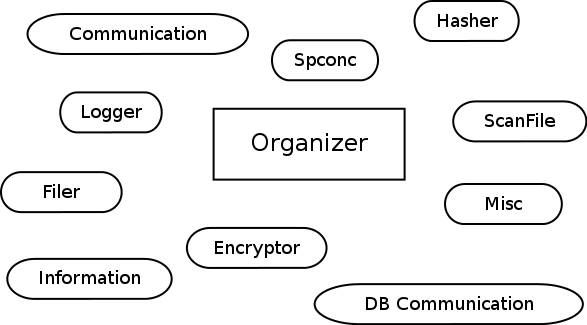
\includegraphics[scale=0.51]{softwareDesign/overviewModule.png}
  \caption{\label{overviewModule} Vue d'ensemble des modules}
\end{figure}

Pour celui-ci, dix modules vont être utilisés autour d'un module central :
\begin{itemize}
  \item \textbf{organizer :} module central qui va créer plus ou moins de
  \textit{thread} et lancer les différents modules nécessaires à la
  sauvegarde ou à la récupération des données.
  \item \textbf{information :} ce module contient les informations
  (méta-informations) nécessaires sur les morceaux de fichiers ainsi que
  sur les fichiers en eux-même.
  \item \textbf{filer :} ce module récupère la liste des fichiers à
  partir du répertoire d'entrée. Il crée les objets correspondants
  (module information) et les transmets au module suivant.
  \item \textbf{spconc :} ce module coupe (\textit{split}) ou concatène ce
  qui lui est envoyé selon qu'il s'agisse d'une sauvegarde ou d'une
  récupération de données.
  \item \textbf{scanFile :} dans le cas où un fichier a déjà été
  sauvegardé, ce module va scanner l'intégralité du fichier pour trouver
  les parties qui ont été modifiées et qui doivent être chiffrées et
  envoyées au serveur.
  \item \textbf{hasher :} ce module fournit des fonction de hachage permettant
  de vérifier l'intégrité des fichiers.
  \item \textbf{encryptor :} ce module s'occupe du chiffrement et du
  déchiffrement des données.
  \item \textbf{communication :} ce module s'occupe de la communication avec
  le serveur.
  \item \textbf{dbcomm :} ce module contient les fonctions utilisées pour la
  communication avec la base de données
  \item \textbf{misc :} ce module contient divers outils
  (\textit{miscellaneous}) pouvant être utile dans le programme. Entre autre
  il contient le système de notification permettant la communication entre
  les différents modules
  \item \textbf{logger :} ce module permet de garder une trace lors de
  l'exécution du programme, notamment utile lors du déboguage ou si une
  erreur provoque l'arrêt prématuré du programme.
\end{itemize}

\subparagraph{}
L'utilisation de modules doit permettre une modification facile du programme,
sans avoir à modifier tout le code. Par exemple, pour changer un algorithme,
il ne doit être nécessaire d'écrire que le code de celui-ci, sans
modifier celui déjà en place. Par la suite, on ne devrait avoir à
préciser que l'algorithme souhaité lors de la création d'un objet.

Un autre avantage de la programmation modulaire est la facilitée que cela
apporte pour maintenir le code efficacement.

Dans ce but, j'utiliserai et profiterai des spécificités qu'offre la
programmation orientée objet.

\subsection{Interaction entre modules}

L'utilisation de \textit{threads} pour exécuter les différents modules
complexifie l'interaction entre ceux-ci. Plusieurs modules sont utilisés
successivement pour pouvoir traiter un fichier, de la lecture depuis le disque
jusqu'à l'envoie des blocs --- chiffrés --- le constituant (dans le cas
d'une sauvegarde). Dans ce sens, les modules doivent communiquer entre eux. Un
lien est donc nécessaire pour que deux \textit{threads} puisse s'envoyer les
données liées à un fichier.

Dans un premier temps, j'avais crée un outil qui, appelé par un module,
retournait un \textit{pipe} (tunnel) soit en lecture, soit en écrite. Un autre
module pouvait ensuite utiliser ce même outil pour récupérer le tunnel.
Un module ayant accès au tunnel en lecture et l'autre en écrite, une
communication peut être effectuée dans un sens. Un second tunnel est
nécessaire pour pouvoir communiquer dans les deux sens. En triant les
tunnels ainsi créés par catégories, il était possible de faire
communiquer deux modules tel que, par exemple, \textit{encryptor} et
\textit{communication}. Le premier pouvait ainsi envoyer ou recevoir des
données vers ou depuis le module \textit{communication}. Dans ce cas, la
catégorie du tunnel aurait alors pu s'appeler \textit{encomm}.

Il y avait néanmoins un problème majeur à l'utilisation d'un tel outil.
Car s'il permettait bien d'envoyer des informations entre deux modules sans
que ceux-ci ne se connaissent, ils ne pouvaient pas envoyer d'objet
\textit{C++}. En somme ils ne pouvaient pas s'envoyer les méta-informations
du fichier sur lequel ils étaient en train de travailler. Ils n'avaient
donc que les octets du fichiers.

Pour palier à ce problème, nous nous sommes donc dirigés vers les patrons
de conception (\textit{design pattern}).

\subsubsection{Design pattern}
\paragraph{Observer\\}
Pour faire ce lien, nous avons dans un premier temps pensé au
\textit{design pattern} \textit{observer}, dont le principe est de notifier des
objets inconnus d'un changement d'état. Dans notre cas, celà aurait permis
que, lors du changement d'état d'un module, les autres modules l'observant
soient avertis et puissent, ou non, agir en conséquence. Cela donne
également la possibilité à un module d'envoyer des informations en
passant dans un certain état à des moments clés. Dans notre cas, elles
auraient correspondu aux méta-données d'un fichier, accompagné d'un
\textit{pipe} servant de tunnel pour faire transiter le fichier en lui-même
d'un \textit{thread} à un autre.

Cette solution ne fut néanmoins pas retenue puisqu'elle impliquait qu'un
module ait connaissances de celui à qui envoyer les informations. Ceci
n'était pas voulu afin de laisser les modules aussi indépendant que
possible.

\paragraph{Event Notifier\\}
Afin d'éviter que certains modules aient connaissances de l'existence d'autres
modules, un système de notification a donc été implémenté. Le
principe de ce système est relativement simple à comprendre. On peut
d'ailleurs trouver le même système dans la vie de tous les jours. Par
exemple un journal publie régulièrement des nouvelles ayant un certain
libellé (\flqq alertes\frqq, \flqq national\frqq, \flqq sport\frqq, etc.).
En face, il existe des utilisateurs qui peuvent, ou non, s'inscrire à un ou
plusieurs type de nouvelle. Ainsi, quelqu'un inscrit aux nouvelles de type
\flqq alertes\frqq~va recevoir une notification lorsqu'une nouvelle de ce type
apparaît.

Le principe utilisé dans notre cas est exactement le même : des modules
lancent des notifications que d'autres reçoivent s'ils se sont inscrits à
celles-ci.

Pour que cela fonctionne correctement, un centre de notification est
nécessaire. Ainsi, et contrairement à un système d'\flqq observer\frqq,
les modules n'ont pas à avoir connaissance les uns des autres puisque chacun
passe par ce centre.

Celui-ci est présenté figure~\ref{classDiagramNotif}. On retrouve le
centre de notification \textit{CNotificationService} qui gère les
abonnements et les abonnés. Ce centre permet ainsi de les notifier les modules
ayant souscrit à un certain type de notification. Pour utiliser ce service,
il existe deux interfaces : \textit{ISubscriber} pour les abonnés et
\textit{INotifier} pour émettre les notifications. Ces interfaces sont donc
implémentée par les différents modules utilisant le système de
notification.

\begin{figure}[h!]
  \hspace{-4.5em}
  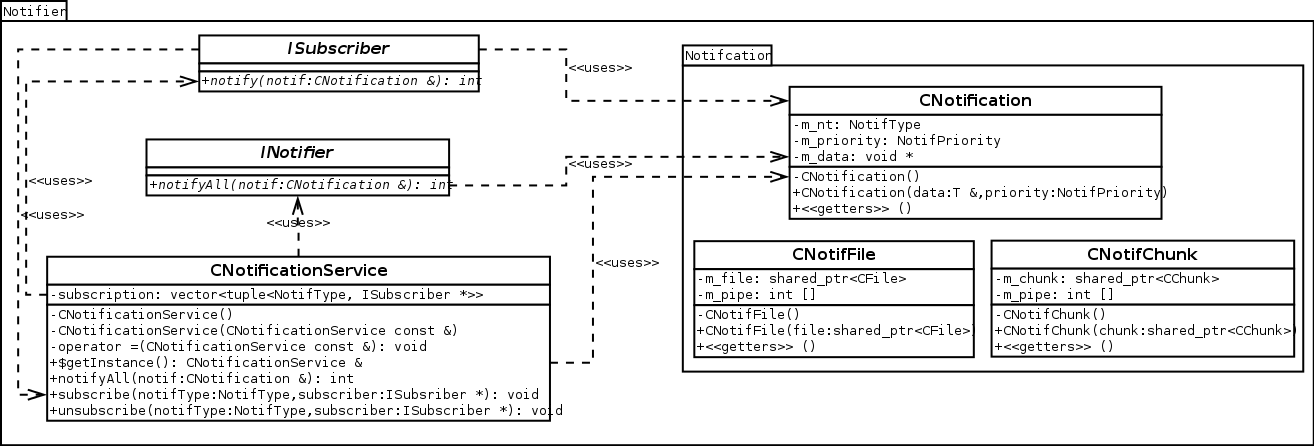
\includegraphics[width=19cm]{softwareDesign/classDiagramNotif.png}
  \caption{\label{classDiagramNotif} Diagramme de classe --- notifications}
\end{figure}

\subparagraph{}
\begin{figure}[h!]
  \hspace{-1.5em}
  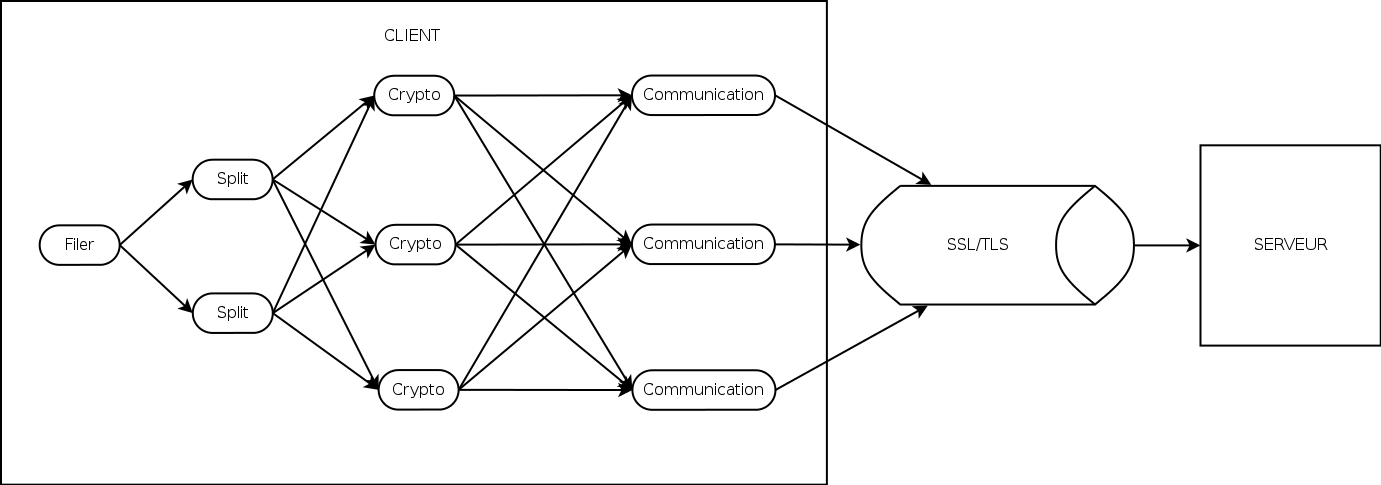
\includegraphics[width=17cm]{softwareDesign/moduleInteraction.png}
  \caption{\label{interactModule} Fonctionnement lors d'une première
  sauvegarde}
\end{figure}

La figure~\ref{interactModule} montre comment le programme fonctionne dans le
cas d'une première sauvegarde sur le serveur. Chaque noeud à l'intérieur
du client est un module exploitant un \textit{thread} différent. Ainsi
avons-nous :
\begin{itemize}
 \item une seule instance de \textit{Filer} est exécutée. Le module
 communique avec une des instances libre du module \textit{Split}, i.e.~qui
 n'est pas déjà en train de travailler sur un fichier
 \item À son tour, le module \textit{Split} communique avec n'importe quel
 \textit{thread} exécutant le module \textit{Crypto} en lui envoyant les
 données à chiffrer.
 \item Enfin, celui-ci envoie les données chiffrées au module
 \textit{Communication} qui va simplement s'occuper de les envoyer sur le
 serveur.
\end{itemize}

\subsection{Base de données}
À la fois du côté client et du côté serveur, l'utilisation d'une
base de données semblait obligatoire afin de garder les méta-données
des fichiers sauvegardés mais également pouvoir garder en mémoire une
trace de chaque sauvegarde effectuée. Cela donnerait la possibilité
de restaurer n'importe quelle version d'un ou plusieurs fichier(s). De ce fait
nous aurions donc l'ensemble des informations nécessaires à la
reconstruction d'une version particulière d'un fichier.

L'utilisation d'une base de donnée côté serveur était donc évidente.
Le choix d'en avoir une également sur la machine cliente s'est fait
naturellement dans la mesure où cela évite d'avoir à effectuer
régulièrement des connexions avec le serveur. Néanmoins, et contrairement
à la base de donnée présente sur le serveur, celle du client permettrait
de ne stocker que les informations liées à la dernière sauvegarde. Ce
sont en effet ces informations qui sont utiles lors d'une nouvelle sauvegarde.
On réduit de ce fait le temps de traitement ainsi que la quantité de
données transmises à travers le réseau Internet.

\subsubsection{SQL vs NoSQL}
La probématique fut donc de trouver quelle type(s) de base de données
pourrai(en)t être utilisé(s) avec d'un côté les bases de données
relationnelle \textit{SQL} et d'un autre les bases de données \textit{NoSQL}.
Les principales différences sont exposées table~\ref{tabSQLNoSQL}.

\begin{savenotes}
\begin{table}[h!]
  \def\arraystretch{1.5}
  \setlength{\fboxsep}{13pt} % padding
  \setlength{\fboxrule}{0pt} % frame
  \begin{tabular}{lm{6cm}m{6cm}}
   \rowcolor{arkred} 
    \arrayrulecolor{gray73}\hline
    & \color{white} \textbf{\textit{SQL}} &
    \color{white} \textbf{\textit{NoSQL}}\\
    Stockage des données & Utilisation d'un modèle relationnel avec les
    traditionnelles lignes et colonnes contenant les différentes entrée de
    la base de données avec l'ensemble des informations correspondantes. &
    Il existe plusieurs modèle de stockage parmi lesquels : documents,
    clé-valeur, graphe, etc.\\
    \hline
    Schéma et flexibilité & Chaque table correspond à un schéma
    particulier. Les colonnes doivent donc être choisie à l'avance, selon
    les données à rentrer dans la table. & Les schéma sont dynamiques.
    Deux entrée d'une même table peuvent contenir différentes
    informations. On peut donc en ajouter \flqq à la volée\frqq\\
    \hline
    Adaptabilité & L'évolutivité est verticale. C'est-à-dire que plus
    la quantité de données augmente, plus le serveur sur lequel se trouvent
    les données doit être important. Ce qui peut engendrer d'important
    coûts & L'évolutivité est horizontale. C'est-à-dire que les
    données peuvent être réparties à travers plusieurs serveurs. Ceux-ci
    sont beaucoup moins onéreux que d'investir dans un très gros serveur.\\
    \hline
    Propriétés ACID\footnote{Atomicité, Cohérence, Isolation,
    Durabilité} & La grande majorité des bases de données relationnelle
    ont ces propriétés & Dépend de la technologie utilisée. Plusieurs
    solution \textit{NoSQL} sacrifie certaines propriétés pour de meilleurs
    performances et une meilleure adaptabilité.\\
  \end{tabular}
  \caption{\label{tabSQLNoSQL} Tableau comparatif \textit{SQL} et
  \textit{NoSQl}}
\end{table}
\end{savenotes}


\subsubsection{Sur le serveur}
Un des principaux points qui nous intéresse est ici l'adaptabilité. En
effet, la quantité de données pouvant augmenter très rapidement il peut
être très coûteux d'utiliser une base de données relationnelle. Cela
signifierait d'importants investissements afin de mettre en place des serveurs
capables de contenir l'intégralité des données.

Le \textit{NoSQL} était donc une solution évidente à ce problème de par
son évolutivité horizontale. De plus cette solution offre également une
réplication des données à travers les différents serveurs. Celle-ci
est d'ailleurs faite automatiquement sur la plupart des solutions
\textit{NoSQL}.

\subsubsection{Sur le client}
Afin d'avoir un accès rapide des informations de la dernière sauvegarde
faite, une base de données doit être installée sur le poste client.

Nous avons dans un premier temps pensé au modèle relationnel avec une base
de données \textit{SQLite} permettant de l'intégrer directement au
programme. Celle-ci étant stockée dans un fichier, et ce indépendemment
de la plate-forme utilisée, elle aurait pu correspondre à ce que voulions.

Néanmoins la quantité d'information stockée ainsi que le nombre d'accès,
tant en écrite qu'en lecture, est trop important dès lors que l'on souhaite
sauvegarder plus de quelques fichiers. Il nous fallait une base de données
avec de meilleurs performances que celles offerte par \textit{SQLite}. De plus
les relations entre les différentes tables étant minimes comme
montré figure~\ref{dbRelClient}, nous pouvions privilégier la performance
du \textit{NoSQL} par rapport aux propriétés ACID qu'offrent le
\textit{SQL}.

Nous avons donc décidé par la suite de nous diriger, comme pour la partie
serveur, sur une base de données \textit{NoSQL}.

\begin{figure}[h!]
  \centering
  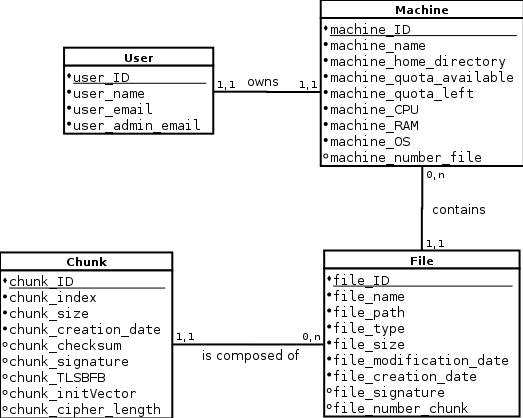
\includegraphics[scale=0.69]{softwareDesign/dbRelClient.png}
  \caption{\label{dbRelClient} Base de données relationnelle --- client}
\end{figure}

La signification des différentes colonnes présentes figure~\ref{dbRelClient}
se trouve en annexe~\ref{annBDR}.

\subsubsection{Choix de la base de données}
En plus des méta-données des différents fichiers sauvegardés, le
stockage des fichiers sur le serveur a influé sur le choix de la base de
données. 

Certaines bases de données \textit{NoSQL} offrent la possibilité de 
sauvegarder les fichiers eux-mêmes. Cela peut être intéressant. que ce
soit dans l'immédiat ou dans une future version de l'application.

Donc bien que dans un premier temps nous ayons décidé d'utiliser le
système de fichier en place sur le serveur, nous avons pris en compte cette
fonctionnalité.

C'est donc sur \textit{MongoDB} que s'est arrêté notre choix. Cette base
de données a plusieurs avantages qui correspondait à ce que nous
recherchions :

\begin{itemize}
 \item Réplication automatique des données sur plusieurs serveurs
 \item Bonne performance
 \item \textit{GridFS} pour stocker de plus grosses quantités d'information
 (correspondant au fichier sauvegardée dans notre cas).
\end{itemize}

C'est également une des bases de données les plus utilisées pour du
\textit{NoSQL}. La communauté, et donc les sources pour rechercher des
informations relatives à son utilisation, est assez importante. N'ayant
jamais utilisé \textit{MongoDB} auparavant il était intéressant, bien que
pas forcément nécessaire, de pouvoir assez facilement accéder à une
possible aide si un problème arrivait.

Le modèle de stockage dans \textit{MongoDB} est de type documents. La
table~\ref{tabMappSQLMongoTerms} présente l'équivalence entre les termes
utilisé pour une base de données \textit{SQL} avec ceux utilisés dans
\textit{MongoDB}. Plus de précisions sont disponible sur le site
\textit{MongoDB}~\cite{refMappingSQLMDB}.

\begin{table}[h!]
  \centering
  \def\arraystretch{1.5}
  \setlength{\fboxsep}{13pt} % padding
  \setlength{\fboxrule}{0pt} % frame
  \begin{tabular}{lm{6cm}m{6cm}}
   \rowcolor{arkred} 
    \arrayrulecolor{gray73}\hline
    \color{white} \textbf{\textit{SQL}} &
    \color{white} \textbf{\textit{MongoDB}}\\
    \hline
    Table & Collection\\
    \hline
    Ligne & Document\\
    \hline
    Colonne & Champ\\
    \hline
    Index & Index\\
    \hline
    Jointure entre tables & Documents intégrés et liés
  \end{tabular}
  \caption{\label{tabMappSQLMongoTerms} Équivalent des termes \textit{SQL}
  avec les termes \textit{MongoDB}}
\end{table}

\subsubsection{Schémas}
Bien que quelque peu différent, les schémas des bases de données
présentes sur le serveur et le client ressemblent à celui présent
figure~\ref{dbRelClient}.

L'absence de relations entre les différentes collections a donc obligé une
modification des schémas. De plus, le serveur doit prendre en compte qu'un
utilisateur peut avoir plusieurs machines alors que le client ne s'occupe que
de la machine sur laquelle il est installé.

\paragraph{Client\\}
Les structures suivantes représentent les collections de la base de données
installée sur les machines clientes.

\begin{lstlisting}[language=json]
User :
{ "_id",
  "username",
  "email",
  "admin_email",
  "machine" :
    { "id_machine",
      "name",
      "home_directory",
      "quota_available",
      "quota_left",
      "CPU",
      "RAM",
      "OS"
    }
}
\end{lstlisting}

On voit ici que l'ancienne table \textit{Machine} a été intégrée dans
la collection \textit{User}. Ce choix s'est fait puisque, sur le client
il n'y a que la machine sur laquelle le logiciel est installé qui est
présente en base de données. De plus, l'accès aux données est à la
fois plus simple et plus rapide en utilisant une collection regroupant
l'utilisateur et sa machine plutôt qu'en utilisant deux collections
distinctes.

\begin{lstlisting}[language=json]
File :
{ "_id",
  "filename",
  "filepath",
  "filetype",
  "filesize",
  "modification_date",
  "creation_date",
  "signature",
  "number_chunk"
}
\end{lstlisting}

N'ayant que les informations d'un seul utilisateur et d'une seule machine,
il n'est pas utile de lier d'une quelconque manière que ce soit la
collection \textit{File} avec la collection \textit{User}.

\begin{lstlisting}[language=json]
Chunk :
{ "_id",
  "id_file"
  "index",
  "size",
  "creation_date",
  "checksum",
  "signature",
  "TLSBFB",
  "init_vector",
  "cipher_length"
}
\end{lstlisting}

Le lien entre la collection \textit{Chunk} et la collection \textit{File} est
représenté par le champ \textit{id\_file} contenant l'identifiant d'un
fichier auquel appartient un morceau.

\paragraph{Serveur\\}
Bien que similaire, la base de données est légèrement différente sur le
serveur par rapport au client. Les changements prennent en compte le fait qu'il
puisse exister plusieurs machines pour un utilisateur mais aussi que plusieurs
utilisateurs existent au sein d'une compagnie.
\begin{lstlisting}[language=json]
User :
{ "_id",
  "id_admin",
  "is_admin",
  "username",
  "email",
  "admin_email",
  "machine" :
    [
      { "id_machine",
	"name",
	"home_directory",
	"quota_available",
	"quota_left",
	"CPU",
	"RAM",
	"OS"
      },
      { "id_machine",
	"name",
	"home_directory",
	"quota_available",
	"quota_left",
	"CPU",
	"RAM",
	"OS"
      },
      ...
    ]
}
\end{lstlisting}
Un utilisateur pouvant avoir plusieurs machines, on crée simplement une
liste  avec l'ensemble des machines qui est intégrée dans la collection
\textit{User}. De plus, un utilisateur pouvant être un administrateur, et
celui-ci pouvant gérer plusieurs utilisateurs, on ajoute un lien à l'aide
du champ \textit{id\_admin}. Ainsi si le champ n'existe pas, l'utilisateur n'a
pas d'administrateur au-dessus de lui. Aussi \textit{is\_admin} permet de
connaître les privilège d'un utilisateur. L'utilisation de ces deux champs
permet donc de prendre compte qu'un administrateur peut lui-même avoir un
autre administrateur au-dessus de lui. Cas que l'on peut imaginer possible dans
le cadre de l'utilisation du logiciel au sein d'une grosse société.

\begin{lstlisting}[language=json]
File :
{ "_id",
  "id_machine",
  "filename",
  "filepath",
  "filetype",
  "filesize",
  "modification_date",
  "creation_date",
  "signature",
  "number_chunk"
}
\end{lstlisting}
Comme plusieurs machines peuvent exister pour un seul utilisateur, on ajoute
le champ \textit{id\_machine} pour pouvoir faire correspondre un fichier à
une seule machine.

\begin{lstlisting}[language=json]
Chunk :
{ "_id",
  "id_file"
  "index",
  "size",
  "creation_date",
  "checksum",
  "signature",
  "TLSBFB",
  "init_vector",
  "cipher_length"
}
\end{lstlisting}

\subsection{Stockage des fichiers}
Comme nous l'avons vu précédemment, \textit{MongoDB} combiné avec
\textit{GridFS} permet de stocker des fichiers. Néanmoins nous avons
décidé d'utiliser, au moins dans un premier temps, le système de fichier
disponible sur le serveur : celui-ci ayant de meilleurs performances en lecture
et écriture.

La figure~\ref{fileSystemServer} présente comment les données seront
stockées sur le serveur une fois sauvegardées. Ainsi chaque fichier
correspond à un dossier contenant un on plusieurs sous-dossier (un par
version). La version d'un fichier correspondant à une sauvegarde à un moment
donné, un dossier contient uniquement parties modifiées du fichier.

\begin{figure}[h!]
  \hspace{-4.5em}
  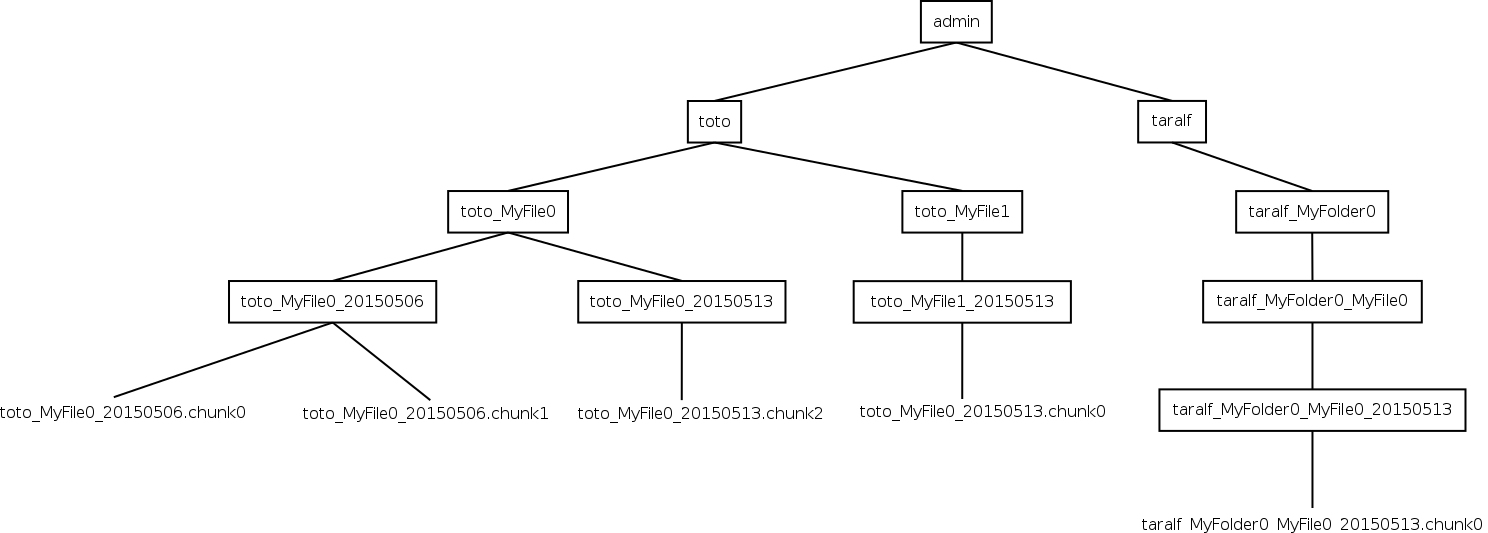
\includegraphics[width=19cm]{softwareDesign/fileSystemServer.png}
  \caption{\label{fileSystemServer} Stockage des fichiers sur le serveur}
\end{figure}

Dans notre exemple, pour récupérer le fichier \textit{MyFile0} de
l'utilisateur \textit{toto}  dans sa version datant du 13 mai 2015, nous devons
donc télécharger \textit{toto\_MyFile0\_20150513.chunk2} mais aussi les
morceaux \textit{.chunk0} et \textit{.chunk1} datant de la précédente
sauvegarde, au 06 mai 2015.

\subsection{Communication client - serveur}
Afin d'envoyer les fichiers à travers le réseau, un protocole doit être
utilisé. Pour ce faire, il m'a été demandé d'en créer un correspondant
aux données qui sont envoyé dans le cadre d'une sauvegarde. En l'occurrence,
les morceaux d'un fichier avec les méta-données correspondantes.

Comme indiqué dans la section \flqq~\nameref{secTravailRecherche} \frqq, je me
suis servi du protocole créé pour \textit{syncthings} (\textit{BEP}).
Celui-ci étant décrit sur le github du projet~\cite{refBEP} et
disponible sous licence Creative Commons~\cite{refCC4.0}, il est autorisé de
le copier, modifier et réutiliser pour n'importe quelle utilisation, même
commerciale. Bien que ce dernier point ne nous concerne pas puisque le projet
sera Open Source, j'ai pu récupérer le protocole et l'adapter pour qu'il
corresponde à nos besoins.

Le protocole ainsi modifié est disponible en annexe~\ref{annProtocolComm}, en
anglais puisqu'également disponible sur le wiki du projet. Celui-ci n'est pas
accessible à l'heure actuelle puisque le projet est toujours dans sa phase de
développement.

\subsection{Algorithme de cryptographie}
À deux reprise il m'a été demandé d'utiliser des algorithme de
cryptographie. Dans un premier temps pour calculer la signature de chaque
fichier et bloc constituant un fichier. Dans un second temps pour chiffrer
ces blocs.

Le premier cas concerne l'utilisation d'un algorithme de hachage alors que dans
le second cas, il est demandé d'utiliser un algorithme de chiffrement
symétrique.

\subsubsection{Algorithme de hachage}
L'idée est d'utiliser la signature pour pouvoir d'une part vérifier
l'intégrité d'un fichier, et d'autre part de repérer un bloc particulier d'un
fichier d'une sauvegarde à l'autre.

C'est notamment le second cas qui nous intéresse puisqu'en utilisant notre
algorithme d'identification de bloc dans un fichier, il sera souvent demandé
de calculer la signature d'un bloc. Il faut donc un algorithme qui soit à la
fois assez fiable pour minimiser le risque de collision, mais rapide à
calculer pour optimiser au mieux notre algorithme lors de son exécution.

\textit{SHA-256}\cite{refSHA256} semblait donc être un bon compromis. Plus
lent à calculer qu'un \textit{SHA-512}, le risque de collision est
inférieur par rapport à un \textit{SHA-128} ou \textit{SHA-224}. Notre
choix s'est donc arrêté sur cet algorithme.

\subsubsection{Algorithme de chiffrement symétrique}
David et Gaëtan avaient déjà dans l'idée d'utiliser
\textit{AES-CBC}\footnote{AES -- Advanced Encryption Standard}\footnote{CBC --
Cipher Block Chaining}\cite{refAES}\cite{refCBC} avec une clé secrète de
256 bits. Cette clé secrète ne serait présente que sur la machine cliente.
Ainsi, le serveur ne contiendrait que des données chiffrées, sans
possibilité de les déchiffrer.

\begin{figure}[h!]
  \centering
  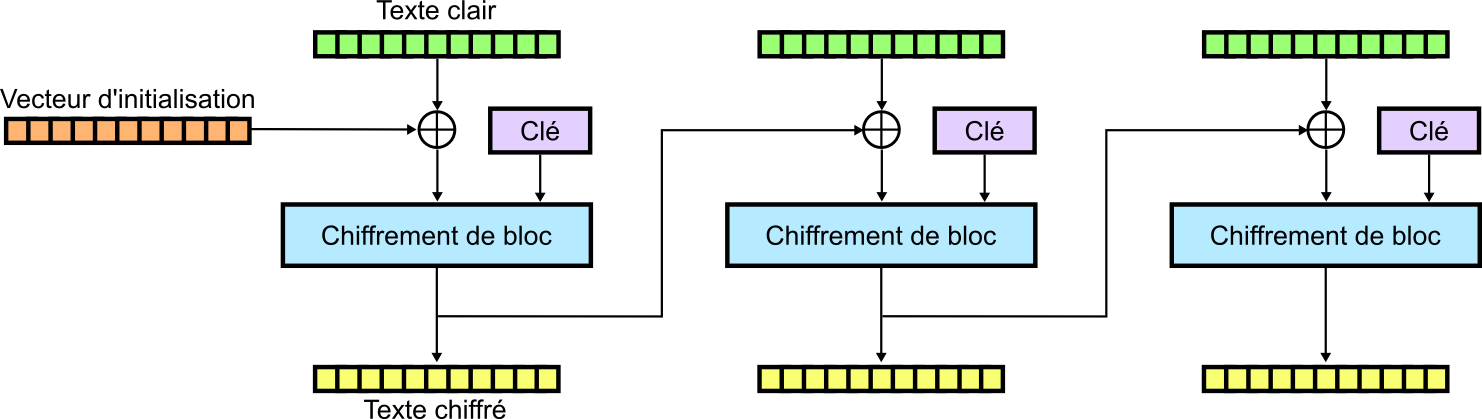
\includegraphics[width=15cm]{softwareDesign/schemaCBC.png}
  \caption{\label{schemaCBC} Comprendre CBC}
\end{figure}

La figure~\ref{schemaCBC} présente le fonctionnement de \textit{CBC}. L'idée
et que, pour chaque calcul d'un bloc de donnée, le résultat chiffré est
utilisé pour calculer le bloc suivant, et ainsi de suite jusqu'à ce que
l'intégralité des données soit chiffré. Un vecteur d'initialisation
est donc utilisé pour chiffrer le tout premier bloc de données.


\section{Développement}
Le client et le serveur étant indépendant l'un de l'autre si ce n'est la
partie communication de l'un à l'autre, le développement se fait tout
aussi indépendemment.

Le client étant la plus grosse partie du système de backup, je me suis
concentré sur son développement durant mon stage. Comme il avait été
découpé en module durant la phase de conception, le développement s'est
fait de la même manière.

De plus chaque module a le droit à sa batterie de tests unitaires et tests de
non régression.

\subsection{Outils de développement}
Pour cette phase j'ai utilisé plusieurs outils me permettant de construire
au mieux l'application demandée. 

Le développement s'est principalement fait dans un environnement
\textit{Unix}. J'ai utilisé \textit{Debian 7} pour le développement de
l'application et comme outil de travail principal. Pouvant avoir accès à un
environnement \textit{Mac OSX} dans l'entreprise, j'ai également pu tester
mon programme sur celui-ci.

La priorité étant d'avoir une première version fonctionnelle du
programme, je n'ai pas porté celui-ci sur un système \textit{Windows}
durant mon stage.

\subsubsection{Environnement de travail}
\begin{itemize}
 \item \textit{vim} comme éditeur de texte
 \item \textit{gcc} comme compilateur
 \item \textit{gdb} pour déboguer le programme quand nécessaire
 \item \textit{valgrind} pour tout ce qui touche à la mémoire (analyse,
 gestion de la mémoire)
 \item \textit{gprof} pour ce qui s'agit de l'analyse de performance
 \item \textit{git} comme gestionnaire de versions décentralisé
\end{itemize}

\subsubsection{Frameworks et bibliothèques externes}
Afin de limiter les contraintes liés à l'utilisation de \textit{framework}
et librairies externes, l'utilisation de ceux-ci était limité. Voici
ceux que j'ai utilisé :
\begin{itemize}
 \item \textit{Boost} pour les tests
 \item \textit{OpenSSL} pour tout ce qui est cryptographie
 \item \textit{Magic} pour récupérer des informations sur les fichiers
 comme le MIME type
\end{itemize}

En addition à cela, j'ai également utilisé le driver \textit{C++} de
\textit{MongoDB} pour communiquer avec la base de données.

Ceux-ci sont tous disponibles pour les environnements \textit{Mac OSX},
\textit{Windows} et \textit{GNU/Linux}.

\subsection{Travail réalisé}
Comme il a été initialement pensé, j'ai développé le système de
sauvegarde module par module, tous indépendant les uns des autres en
préférant dans un premier temps la partie principale du programme. Cette
partie correspond à la lecture des fichiers depuis le disque, le découpage
en morceaux ainsi que le chiffrement de ceux-ci.

\subsubsection{Développement des modules}
J'ai donc tout d'abord créé le \textit{logger} qui allait m'aider, pendant
l'ensemble du développement du programme, à déceler plus facilement les
problèmes pouvant exister.

Une fois ceci fait, j'ai développé toute la partie concernant la
cryptographie. Cette partie comprend les modules \textit{hasher} et
\textit{encryptor}. J'ai utilisé les méthodes fournies par la bibliothèque
\textit{OpenSSL} afin d'écrire ces deux modules. L'utilisation de méthodes
déjà existantes étant préférable à la réécriture de celles-ci.
Le risque de bogues et de failles étant limité dans le premier cas.

S'en est suivi le développement du module \textit{spconc}, permettant dans un
sens de découper en plusieurs morceaux un fichier, ou à l'inverse de
concaténer ces morceaux pour retrouver le fichier d'origine.

Après celui-ci, ce fut autour du module \textit{information} d'être
développé afin de pouvoir créer des objets permettant de garder les
méta-données des fichiers.

À partir de là, nous avions assez de module combinables afin de lancer le
programme dans sa toute première phase d'essai. Pour simuler une sauvegarde,
il manquait des prototypes pour mimer le rôle des modules \textit{filer},
\textit{communication} et \textit{organizer}. En plus de cela, il nous fallait
bien évidemment développer le système de notification pour pouvoir faire
communiquer les différents modules.

Une fois ceci fait, je pouvais créer l'\textit{organizer} afin de faire
fonctionner tous ces modules ensemble.

\subsubsection{Imbrication des modules}
Cette étape fut longue et beaucoup d'erreurs apparurent. Bien que chaque
module, individuellement, fonctionnait parfaitement, l'exécution sur des 
threads séparés, ainsi que la communication entre eux amena plusieurs
problèmes.

\paragraph{Problèmes et solutions}

\subparagraph{Chiffrement et déchiffrement\\}
Un des points sur lequel j'ai passé le plus de temps a été la partie
chiffrement et déchiffrement. Car si le programme n'émettait pas d'erreurs
dans le cas du chiffrement, les morceaux créés en sortie ne correspondaient
pas à ce que l'on pouvait attendre.

Bien qu'ayant préciser dans le code du programme que je voulais écrire
sur le disque du binaire et non des caractères ASCII, il semblait que
l'utilisation des \textit{iofstream} (flux d'entrée/sortie sur des fichiers)
posait problèmes. En effet, un nombre aléatoire de caractère était
écrit dans les fichiers de sortis. 

De par ce fait, il était tout simplement impossible de reconstruire les
fichiers proprement puisqu'il était impossible alors de les déchiffrer.

La solution a été l'utilisation des \textit{FILE}\footnote{Structure
permettant de contenir les informations nécessaire au contrôle d'un
flux~\cite{refFILE}} du \textit{C} pour tout ce qui est gestion de fichiers en
lieu et place des \textit{iofstream}\footnote{Classes (
\textit{ifstream}~\cite{refIFS} et \textit{ofstream}~\cite{refOFS}) gérant
des flux en entrée ou en sortie pour travailler sur des fichiers} du
\textit{C++}.

\subparagraph{Problèmes de mémoire\\}
Avec l'utilisation du \textit{C++}, je devais gérer moi-même l'utilisation
de la mémoire. J'ai donc rencontré deux soucis : fuites de mémoire et
libération précipitée de la mémoire.

Dans le premier cas, il suffisait simplement de libérer la mémoire au bon
moment. C'est-à-dire lorsqu'il n'est plus utile d'accéder à la mémoire
allouée précédemment dans le programme.

En ce qui concerne le second cas, cela posait problème puisque plusieurs
\textit{threads} tournaient en parallèles. Ainsi était-ce au rôle du
\textit{thread} ayant alloué la mémoire de la libérer. Néanmoins,
d'autres modules, exécutés sur d'autres \textit{threads}, pouvaient utiliser
cette même mémoire. C'était notamment le cas des objets contenant les
méta-informations des fichiers. Si le premier module libérait la mémoire
allouée, il devenait impossible pour les suivants d'utiliser cette mémoire
qui ne contenait alors plus l'objet voulu.

Pour résoudre ce problème deux solutions s'offraient à moi :
\begin{itemize}
 \item La première était de libérer la mémoire une fois que tout les
 modules l'utilisant avait finit leur exécution sur l'objet contenu dans cet
 espace mémoire.
 \item La seconde était d'utiliser des pointeurs intelligents. Ceux-ci
 fonctionnent de la même faç qu'un \textit{garbage collector}
 (ramasse-miettes)\footnote{ Sous-système informatique de gestion automatique
 de la mémoire. Il est responsable du recyclage de la mémoire
 préalablement allouée puis inutilisée} : tant que la mémoire est
 utilisée, elle n'est pas libérée ; elle est libérée automatiquement
 lorsqu'elle n'est plus utilisé, dans aucun module.
\end{itemize}

La seconde solution était bien évidemment préférable puisqu'elle
réglait aussi les soucis de fuites de mémoire pouvant exister çà et
là dans le programme.

\paragraph{Ajout des fonctionnalités}
Une fois toutes les erreurs corrigées, nous avions une version fonctionnelle
du programme. Cette version permettait de chiffrer un fichier (que l'on
précisait dans un premier temps en début d'exécution) ainsi que de le
déchiffrer. Les morceaux du fichier ainsi créés et chiffrés étaient
stockés en local sur le disque dur afin de \flqq simuler\frqq~le module
\textit{communication}.

À partir de là il ne restait plus qu'à rajouter les différentes
fonctionnalités nécessaire au bon fonctionnement du programme tel qu'il
avait été demandé.

J'ai donc tout d'abord ajouté la possibilité de lire un dossier de
manière récursive au lieu de lire uniquement un simple fichier. Quelques
petites erreurs que je n'avais pas détecté lors de la précédente
version du programme sont apparues. Entre autres, et principalement, tous les
descripteurs de fichiers\footnote{Un descripteur de fichier est une clé
abstraite pour accéder à un fichier.} ouvert n'étaient pas forcément
fermés. Cela amenait le programme à planter à cause d'un trop grand
nombre de descripteur ouvert. J'ai donc du les fermer pour que le programme
puisse s'exécuter sans problèmes.

À ce moment j'ai testé le programme sur \textit{Mac OSX}. Une erreur de
liaison avec les bibliothèques utilisées empêchait la compilation. Une
simple modification du \textit{Makefile}\footnote{Fichier(s) permettant de
compiler et lier un programme avec les bibliothèques utilisées.} a permis
de résoudre ce léger souci. Le programme pouvait ainsi tourner sur le
système d'exploitation d'\textit{Apple}.

\paragraph{Travail à venir}

L'étape suivante consistait à ajouter la base de données, nécessaire
pour pouvoir intégrer au programme l'algorithme trouvé en tout début de
stage (voir section \flqq~\nameref{secTravailRecherche}~\frqq).

Ne connaissant pas \textit{MongoDB}, je me suis donc formé pour comprendre
comment celui-ci fonctionnait ainsi que pour l'utiliser dans un programme en
\textit{C++}. De plus, un cours en ligne commençant gratuitement sur le site
\flqq\textit{University}\frqq~de \textit{MongoDB}\cite{refMongoDBUniversity},
j'ai suivi ce cours montrant et expliquant comment utiliser \textit{MongoDB}
pour un développeur. Même si le langage utilisé dans le cours est
\textit{Python}, le principe reste le même et je peux réutiliser ce que
j'apprends dans ce cours en adaptant pour le projet de système de sauvegarde.

Au moment d'écrire le rapport j'en suis donc à cette étape là. Une fois
la base de données ajoutée ainsi que le prototype de l'algorithme
intégré dans le programme, il ne restera plus qu'à détecter quels
fichiers ont été modifié depuis la précédente sauvegarde avant de
pouvoir faire tourner le programme pour ne prendre en compte que ces fichiers
là et les analyser, ainsi que les fichiers nouvellement créés.

\subsection{Tests}
Une suite de test unitaires a été écrite pour chaque module. Ainsi est
faite la vérification de chaque méthode de chaque classe de chaque module
dans la mesure du possible. En effet, et c'est notamment vrai pour ce qui touche
aux \textit{threads}, il est parfois difficile d'écrire des tests permettant
de couvrir l'ensemble des cas pouvant exister.

Afin de réaliser les tests, j'ai utilisé le framework de test
\textit{Boost}. Celui-ci m'a donc permis de valider le bon fonctionnement des
différents éléments constituant le programme.

Ces tests ont été écrits au fur et à mesure de l'avancement du projet.
De plus, pour chaque test, une vérification de l'utilisation de la mémoire
était effectuée à l'aide de l'outil \textit{valgrind}. Cela me permettait
de vérifier la présence, ou non, de fuites de mémoire. Je pouvais par la
suite et si nécessaire apporter des modifications au programme.

\chapter{Conclusion}
Ce stage de fin d'étude m'a permis d'acquérir de l'expérience sur
plusieurs points, que ce soit au niveau du développement d'un produit ou du
développement et de la vie dans une startup.

En effet, j'ai dû, au cours de ce stage, concevoir puis développer un
logiciel. Ces étapes commencent la vie du logiciel et sont cruciales pour les
étapes suivante et notamment la maintenance. J'avais ainsi toujours à
l'esprit que l'importance de la documentation, de même que la qualité de
celle-ci et du code. Ceci étant d'autant plus vrai qu'il est prévu que le
code soit distribué sous licence publique. Cela me permettra également de
continuer à travailler dessus une fois le stage terminé.

J'ai donc pu mettre en pratique l'enseignement reçu durant mes cinq années
d'étude, que ce soit à l'IUT, à la faculté des sciences de
l'université d'Aix-Marseille ou à l'université d'Uppsala.

Le plan de restructuration effectué au sein de l'entreprise a aussi été
source d'expérience même si, étant stagiaire, cela ne m'a pas autant
touché que les autres employés de la compagnie. Néanmoins, il est
représentatif de ce qu'il se passe dans de nombreuses startup mais aussi de
ce qu'il peut se passer dans des entreprises de taille plus importante.

De plus, ce stage a été pour moi l'occasion de travailler avec des personnes
de culture et pays différents. Faisant ce stage à l'étranger, j'ai donc
régulièrement dû m'adapter à la culture locale, que ce soit durant mes
heures de travail ou en dehors de celui-ci.

Bien qu'un contrat en CDI était originalement prévu, sous réserve que
l'entreprise veuille me garder et que j'accepte de rester, celui-ci n'était
plus d'actualité à la fin du stage suite à la restructuration effectuée.

Ce stage a donc été une bonne expérience pour moi et va m'être utile par
la suite autant sur le plan professionnel que personnel.

\newpage
\listoffigures
\listoftables
\bibliographystyle{abbrv-fr}
\bibliography{rapport_stage_arksens_2015}

\appendix
\makeatletter
\def\@seccntformat#1{Annexe~\csname the#1\endcsname:\quad}
\makeatother
\part{Annexes}
\chapter{Base de données relationnelle}
\thispagestyle{fancy}
\label{annBDR}
\thispagestyle{fancy}
\section{User}
\begin{table}[h!]
  \centering
  \def\arraystretch{1.5}
  \setlength{\fboxsep}{13pt} % padding
  \setlength{\fboxrule}{0pt} % frame
  \begin{tabular}{lm{6cm}m{6cm}}
   \rowcolor{arkred} 
    \arrayrulecolor{gray73}\hline
    \color{white} \textbf{Colonne} & \color{white} \textbf{Information}\\
    \hline
    user\_id & Identifiant unique pour l'utilisateur\\
    \hline
    user\_name & Nom de l'utilisateur\\
    \hline
    user\_email & Email de l'utilisateur\\
    \hline
    user\_admin\_email & Email de l'administrateur en charge de l'utilisateur.
    Utilisé pour prévenir automatiquement l'administrateur en cas de
    problème de fonctionnement.
  \end{tabular}
  \caption{\label{tabDBRUser} Information colonnes -- User}
\end{table}

\section{Machine}
\begin{table}[h!]
  \centering
  \def\arraystretch{1.5}
  \setlength{\fboxsep}{13pt} % padding
  \setlength{\fboxrule}{0pt} % frame
  \begin{tabular}{lm{6cm}m{6cm}}
   \rowcolor{arkred} 
    \arrayrulecolor{gray73}\hline
    \color{white} \textbf{Colonne} & \color{white} \textbf{Information}\\
    \hline
    machine\_id & Identifiant unique pour la machine\\
    \hline
    machine\_name & Nom de la machine\\
    \hline
    machine\_home\_directory & Répertoire racine des fichiers à
    sauvegarder\\
    \hline
    machine\_quota\_available & Quota disponible (total) pour la machine\\
    \hline
    machine\_quota\_left & Quota restant pour la machine\\
    \hline
    machine\_CPU & Informations relatives au processeur utilisé\\
    \hline
    machine\_RAM & Quantité de RAM disponible\\
    \hline
    machine\_OS & Système d'exploitation utilisé\\
    \hline
    machine\_number\_file & Nombre de fichier sauvegardé
  \end{tabular}
  \caption{\label{tabDBRMachine} Information colonnes -- Machine}
\end{table}

\section{File}
\begin{table}[h!]
  \centering
  \def\arraystretch{1.5}
  \setlength{\fboxsep}{13pt} % padding
  \setlength{\fboxrule}{0pt} % frame
  \begin{tabular}{lm{6cm}m{6cm}}
   \rowcolor{arkred} 
    \arrayrulecolor{gray73}\hline
    \color{white} \textbf{Colonne} & \color{white} \textbf{Information}\\
    \hline
    file\_id & Identifiant unique du fichier\\
    \hline
    file\_name & Nom du fichier\\
    \hline
    file\_path & Chemin du fichier en local\\
    \hline
    file\_type & Type du fichier\\
    \hline
    file\_size & Taille du fichier en octet\\
    \hline
    file\_modification\_date & Date de dernière modification\\
    \hline
    file\_creation\_date & Date de création\\
    \hline
    file\_signature & Signature numérique\\
    \hline
    file\_number\_chunk & Nombre de morceau composant le fichier
  \end{tabular}
  \caption{\label{tabDBRFile} Information colonnes -- File}
\end{table}

\section{Chunk}
\begin{savenotes}
\begin{table}[h!]
  \centering
  \def\arraystretch{1.5}
  \setlength{\fboxsep}{13pt} % padding
  \setlength{\fboxrule}{0pt} % frame
  \begin{tabular}{lm{6cm}m{6cm}}
   \rowcolor{arkred} 
    \arrayrulecolor{gray73}\hline
    \color{white} \textbf{Colonne} & \color{white} \textbf{Information}\\
    \hline
    chunk\_id & Identifiant unique d'un morceau de fichier\\
    \hline
    chunk\_index & Index du morceau de fichier\\
    \hline
    chunk\_size & Taille du morceau en octet\\
    \hline
    chunk\_creation\_date & Date de création\\
    \hline
    chunk\_checksum & Checksum\\
    \hline
    chunk\_signature & Signature numérique\\
    \hline
    chunk\_TLSBFB\footnote{Two Last Significant Bit of First Byte} & Deux bits
    de poids faible du premier octet du morceau. Utilisé pour répartir le
    travail entre plusieurs thread lors du scan d'un fichier pour trouver les
    parties modifiés de celui-ci.\\
    \hline chunk\_init\_vector & Vecteur d'initialisation utilisé pour
    l'algorithme de chiffrement AES\\
    \hline
    chunk\_cipher\_length & Taille du morceau chiffré en octet\\
  \end{tabular}
  \caption{\label{tabDBRChunk} Information colonnes -- Chunk}
\end{table}
\end{savenotes}


\chapter{Protocole de communication}
\thispagestyle{fancy}
\label{annProtocolComm}
\thispagestyle{fancy}
\section{Definition}

The key words "MUST", "MUST NOT", "REQUIRED", "SHALL", "SHALL NOT",
"SHOULD", "SHOULD NOT", "RECOMMENDED", "MAY", and "OPTIONAL" in this
document are to be interpreted as described in RFC 2119.


\section{Transport and Authentication}

This protocol is deployed as the highest level in a protocol stack, with
the lower level protocols providing additional encryption and authentication.

\begin{verbatim}
           +-----------------------------|
           |   Block Exchange Protocol   |
           |-----------------------------|
           | Encryption & Auth (TLS 1.2) |
           |-----------------------------|
           |             TCP             |
           |-----------------------------|
           v             ...             v
\end{verbatim}

\section{Messages}

Every message starts with one 32 bit word indicating the message version,
type and ID, followed by the length of the message. The header is in
network byte order, i.e. big endian.

\begin{itemize}
 \item Message Structure:
\end{itemize}

\begin{verbatim}
            O                   1                   2                   3
            O 1 2 3 4 5 6 7 8 9 0 1 2 3 4 5 6 7 8 9 0 1 2 3 4 5 6 7 8 9 0 1
           +-+-+-+-+-+-+-+-+-+-+-+-+-+-+-+-+-+-+-+-+-+-+-+-+-+-+-+-+-+-+-+-+
           |  Ver  |       Message ID      |      Type     |    Reserved   |
           +-+-+-+-+-+-+-+-+-+-+-+-+-+-+-+-+-+-+-+-+-+-+-+-+-+-+-+-+-+-+-+-+
           |                            Length                             |
           +-+-+-+-+-+-+-+-+-+-+-+-+-+-+-+-+-+-+-+-+-+-+-+-+-+-+-+-+-+-+-+-+
\end{verbatim}

For version 1 the Version field is set to zero. Future versions with
incompatible message formats will increment the Version field. A
message with an unknown version is a protocol error and MUST result
in the connection being terminated. A client supporting multiple
versions MAY retry with a different protocol version upon disconnection.

The Message ID is set to a unique value for each transmitted request
message. In response messages it is set to the Message ID of the
corresponding request message. The uniqueness requirement implies that
no more than 4096 messages may be outstanding at any given moment. The
ordering requirement implies that a response to a given message ID also
means that all preceding messages have been received, specifically
those which do not otherwise demand a response. Hence their message
ID:s may be reused.

The Type field indicates the type of data following the message header
and is one of the integers defined below. A message of an unknown type
is a protocol error and MUST result in the connection being terminated.


\section{Types}
\subsection{0 - Client Config}

This informational message provides information about the client
configuration as it pertains to the current connection. A Client
Config message MUST be the first message sent on a connection.
Additional Client Config messages MUST NOT be sent after the initial
exchange.

\begin{itemize}
 \item ClientConfigMessage Structure:
\end{itemize}

\begin{verbatim}
            O                   1                   2                   3
            O 1 2 3 4 5 6 7 8 9 0 1 2 3 4 5 6 7 8 9 0 1 2 3 4 5 6 7 8 9 0 1
           +-+-+-+-+-+-+-+-+-+-+-+-+-+-+-+-+-+-+-+-+-+-+-+-+-+-+-+-+-+-+-+-+
           |                     Length of ClientName                      |
           +-+-+-+-+-+-+-+-+-+-+-+-+-+-+-+-+-+-+-+-+-+-+-+-+-+-+-+-+-+-+-+-+
           /                                                               /
           \                 ClientName (variable length)                  \
           /                                                               /
           +-+-+-+-+-+-+-+-+-+-+-+-+-+-+-+-+-+-+-+-+-+-+-+-+-+-+-+-+-+-+-+-+
           |                    Length of ClientVersion                    |
           +-+-+-+-+-+-+-+-+-+-+-+-+-+-+-+-+-+-+-+-+-+-+-+-+-+-+-+-+-+-+-+-+
           /                                                               /
           \                ClientVersion (variable length)                \
           /                                                               /
           +-+-+-+-+-+-+-+-+-+-+-+-+-+-+-+-+-+-+-+-+-+-+-+-+-+-+-+-+-+-+-+-+
           |                       Number of Folders                       |
           +-+-+-+-+-+-+-+-+-+-+-+-+-+-+-+-+-+-+-+-+-+-+-+-+-+-+-+-+-+-+-+-+
           /                                                               /
           \                Zero or more Folder Structures                 \
           /                                                               /
           +-+-+-+-+-+-+-+-+-+-+-+-+-+-+-+-+-+-+-+-+-+-+-+-+-+-+-+-+-+-+-+-+
           |                       Number of Options                       |
           +-+-+-+-+-+-+-+-+-+-+-+-+-+-+-+-+-+-+-+-+-+-+-+-+-+-+-+-+-+-+-+-+
           /                                                               /
           \                Zero or more Option Structures                 \
           /                                                               /
           +-+-+-+-+-+-+-+-+-+-+-+-+-+-+-+-+-+-+-+-+-+-+-+-+-+-+-+-+-+-+-+-+
\end{verbatim}

\begin{itemize}
 \item Folder Structure:
\end{itemize}

\begin{verbatim}
            O                   1                   2                   3
            O 1 2 3 4 5 6 7 8 9 0 1 2 3 4 5 6 7 8 9 0 1 2 3 4 5 6 7 8 9 0 1
           +-+-+-+-+-+-+-+-+-+-+-+-+-+-+-+-+-+-+-+-+-+-+-+-+-+-+-+-+-+-+-+-+
           |                         Length of ID                          |
           +-+-+-+-+-+-+-+-+-+-+-+-+-+-+-+-+-+-+-+-+-+-+-+-+-+-+-+-+-+-+-+-+
           /                                                               /
           \                     ID (variable length)                      \
           /                                                               /
           +-+-+-+-+-+-+-+-+-+-+-+-+-+-+-+-+-+-+-+-+-+-+-+-+-+-+-+-+-+-+-+-+
           |                       Number of Folders                       |
           +-+-+-+-+-+-+-+-+-+-+-+-+-+-+-+-+-+-+-+-+-+-+-+-+-+-+-+-+-+-+-+-+
           /                                                               /
           \                Zero or more Folder Structures                 \
           /                                                               /
           +-+-+-+-+-+-+-+-+-+-+-+-+-+-+-+-+-+-+-+-+-+-+-+-+-+-+-+-+-+-+-+-+
\end{verbatim}

\begin{itemize}
 \item Option Structure:
\end{itemize}

\begin{verbatim}
            O                   1                   2                   3
            O 1 2 3 4 5 6 7 8 9 0 1 2 3 4 5 6 7 8 9 0 1 2 3 4 5 6 7 8 9 0 1
           +-+-+-+-+-+-+-+-+-+-+-+-+-+-+-+-+-+-+-+-+-+-+-+-+-+-+-+-+-+-+-+-+
           |                         Length of Key                         |
           +-+-+-+-+-+-+-+-+-+-+-+-+-+-+-+-+-+-+-+-+-+-+-+-+-+-+-+-+-+-+-+-+
           /                                                               /
           \                     Key (variable length)                     \
           /                                                               /
           +-+-+-+-+-+-+-+-+-+-+-+-+-+-+-+-+-+-+-+-+-+-+-+-+-+-+-+-+-+-+-+-+
           |                        Length of Value                        |
           +-+-+-+-+-+-+-+-+-+-+-+-+-+-+-+-+-+-+-+-+-+-+-+-+-+-+-+-+-+-+-+-+
           /                                                               /
           \                    Value (variable length)                    \
           /                                                               /
           +-+-+-+-+-+-+-+-+-+-+-+-+-+-+-+-+-+-+-+-+-+-+-+-+-+-+-+-+-+-+-+-+
\end{verbatim}

The ClientName and ClientVersion fields identify the implementation.
The values SHOULD be simple strings identifying the implementation name,
as a user would expect to see it, and the version string in the same
manner. An example ClientName is "acs" and an example ClientVersion is
"v0.7.2". The ClientVersion field SHOULD follow the patterns laid out
in the [Semantic Versioning](http://semver.org/) standard.

The Folders field lists all folders that will be synchronized over the
current connection. Each folder has a list of sub-folders.

The Options field contain option values to be used in an implementation
specific manner. The options list is conceptually a map of Key => Value
items, although it is transmitted in the form of a list of (Key, Value)
pairs, both of string type. Key ID:s are implementation specific. An
implementation MUST ignore unknown keys. An implementation MAY impose
limits on the length keys and values. The options list may be used to
inform of relevant information such as quota and other user information
for example.

\subsection{1 - Index \&\& 7 - Index Update}

This TypeMessages will be used for Client -> Server communication,
i.e.~the actual backup.

The Index and Index Update messages define the contents of the senders
folder. An Index message represents the full contents of the folder and
thus supersedes any previous index. An Index Update amends an existing
index with new information, not affecting any entries not included in
the message.

An Index or Index Update message MUST be sent for each folder included
in the Client Config message, and MUST be sent before any other message
referring to that folder. If the folder contents change from non-empty
to empty, an empty Index message MUST be sent. There is no response to
the Index message.

\begin{itemize}
 \item IndexMessage Structure: 
\end{itemize}

\begin{verbatim}
            O                   1                   2                   3
            O 1 2 3 4 5 6 7 8 9 0 1 2 3 4 5 6 7 8 9 0 1 2 3 4 5 6 7 8 9 0 1
           +-+-+-+-+-+-+-+-+-+-+-+-+-+-+-+-+-+-+-+-+-+-+-+-+-+-+-+-+-+-+-+-+
           |                       Length of Folder                        |
           +-+-+-+-+-+-+-+-+-+-+-+-+-+-+-+-+-+-+-+-+-+-+-+-+-+-+-+-+-+-+-+-+
           /                                                               /
           \                   Folder (variable length)                    \
           /                                                               /
           +-+-+-+-+-+-+-+-+-+-+-+-+-+-+-+-+-+-+-+-+-+-+-+-+-+-+-+-+-+-+-+-+
           |                        Number of Files                        |
           +-+-+-+-+-+-+-+-+-+-+-+-+-+-+-+-+-+-+-+-+-+-+-+-+-+-+-+-+-+-+-+-+
           /                                                               /
           \               Zero or more FileInfo Structures                \
           /                                                               /
           +-+-+-+-+-+-+-+-+-+-+-+-+-+-+-+-+-+-+-+-+-+-+-+-+-+-+-+-+-+-+-+-+
\end{verbatim}

\begin{itemize}
 \item FileInfo Structure:
\end{itemize}

\begin{verbatim}
            O                   1                   2                   3
            O 1 2 3 4 5 6 7 8 9 0 1 2 3 4 5 6 7 8 9 0 1 2 3 4 5 6 7 8 9 0 1
           +-+-+-+-+-+-+-+-+-+-+-+-+-+-+-+-+-+-+-+-+-+-+-+-+-+-+-+-+-+-+-+-+
           |                         Length of ID                          |
           +-+-+-+-+-+-+-+-+-+-+-+-+-+-+-+-+-+-+-+-+-+-+-+-+-+-+-+-+-+-+-+-+
           /                                                               /
           \                     ID (variable length)                      \
           /                                                               /
           +-+-+-+-+-+-+-+-+-+-+-+-+-+-+-+-+-+-+-+-+-+-+-+-+-+-+-+-+-+-+-+-+
           |                        Length of Name                         |
           +-+-+-+-+-+-+-+-+-+-+-+-+-+-+-+-+-+-+-+-+-+-+-+-+-+-+-+-+-+-+-+-+
           /                                                               /
           \                    Name (variable length)                     \
           /                                                               /
           +-+-+-+-+-+-+-+-+-+-+-+-+-+-+-+-+-+-+-+-+-+-+-+-+-+-+-+-+-+-+-+-+
           |                                                               |
           +                      Modified (64 bits)                       +
           |                                                               |
           +-+-+-+-+-+-+-+-+-+-+-+-+-+-+-+-+-+-+-+-+-+-+-+-+-+-+-+-+-+-+-+-+
           |                       Number of Blocks                        |
           +-+-+-+-+-+-+-+-+-+-+-+-+-+-+-+-+-+-+-+-+-+-+-+-+-+-+-+-+-+-+-+-+
           /                                                               /
           \               Zero or more BlockInfo Structures               \
           /                                                               /
           +-+-+-+-+-+-+-+-+-+-+-+-+-+-+-+-+-+-+-+-+-+-+-+-+-+-+-+-+-+-+-+-+
\end{verbatim}

\begin{itemize}
 \item BlockInfo Structure:
\end{itemize}

\begin{verbatim}
            O                   1                   2                   3
            O 1 2 3 4 5 6 7 8 9 0 1 2 3 4 5 6 7 8 9 0 1 2 3 4 5 6 7 8 9 0 1
           +-+-+-+-+-+-+-+-+-+-+-+-+-+-+-+-+-+-+-+-+-+-+-+-+-+-+-+-+-+-+-+-+
           |                             Size                              |
           +-+-+-+-+-+-+-+-+-+-+-+-+-+-+-+-+-+-+-+-+-+-+-+-+-+-+-+-+-+-+-+-+
           |lsb|                        Reserved                           |
           +-+-+-+-+-+-+-+-+-+-+-+-+-+-+-+-+-+-+-+-+-+-+-+-+-+-+-+-+-+-+-+-+
           |                      Length of Signature                      |
           +-+-+-+-+-+-+-+-+-+-+-+-+-+-+-+-+-+-+-+-+-+-+-+-+-+-+-+-+-+-+-+-+
           /                                                               /
           \                  Signature (variable length)                  \
           /                                                               /
           +-+-+-+-+-+-+-+-+-+-+-+-+-+-+-+-+-+-+-+-+-+-+-+-+-+-+-+-+-+-+-+-+
           |                      Length of Checksum                       |
           +-+-+-+-+-+-+-+-+-+-+-+-+-+-+-+-+-+-+-+-+-+-+-+-+-+-+-+-+-+-+-+-+
           /                                                               /
           \                   Checksum (variable length)                  \
           /                                                               /
           +-+-+-+-+-+-+-+-+-+-+-+-+-+-+-+-+-+-+-+-+-+-+-+-+-+-+-+-+-+-+-+-+
           |                          Block Index                          |
           +-+-+-+-+-+-+-+-+-+-+-+-+-+-+-+-+-+-+-+-+-+-+-+-+-+-+-+-+-+-+-+-+
           |                        Length of Data                         |
           +-+-+-+-+-+-+-+-+-+-+-+-+-+-+-+-+-+-+-+-+-+-+-+-+-+-+-+-+-+-+-+-+
           /                                                               /
           \                    Data (variable length)                     \
           /                                                               /
           +-+-+-+-+-+-+-+-+-+-+-+-+-+-+-+-+-+-+-+-+-+-+-+-+-+-+-+-+-+-+-+-+
\end{verbatim}

The Folder field identifies the folder that the index message pertains
to.

The Name is the file name path relative to the folder root. Like all
strings, the Name is always in UTF-8 NFC regardless of operating system
or file system specific conventions. The Name field uses the slash
character ("/") as path separator, regardless of the implementation's
operating system conventions. The combination of Folder and Name
identifies each file on a Client machine as well as a unique ID
specified by Adhara.

The Modified time is expressed as the number of seconds since the Unix
Epoch (1970-01-01 00:00:00 UTC).

The Blocks list contains the size, signature, checksum, block index
and the two least significant bit of the first byte of the block (lsb)
for each block in the file.

\subsection{2 - Request}

The Request message expresses the desire to retrieve a file from the
server or to get the data on modified files to synchronize.

\begin{itemize}
 \item RequestMessage Structure:
\end{itemize}

\begin{verbatim}
            O                   1                   2                   3
            O 1 2 3 4 5 6 7 8 9 0 1 2 3 4 5 6 7 8 9 0 1 2 3 4 5 6 7 8 9 0 1
           +-+-+-+-+-+-+-+-+-+-+-+-+-+-+-+-+-+-+-+-+-+-+-+-+-+-+-+-+-+-+-+-+
           |                       Length of Folder                        |
           +-+-+-+-+-+-+-+-+-+-+-+-+-+-+-+-+-+-+-+-+-+-+-+-+-+-+-+-+-+-+-+-+
           /                                                               /
           \                   Folder (variable length)                    \
           /                                                               /
           +-+-+-+-+-+-+-+-+-+-+-+-+-+-+-+-+-+-+-+-+-+-+-+-+-+-+-+-+-+-+-+-+
           |                        Length of Name                         |
           +-+-+-+-+-+-+-+-+-+-+-+-+-+-+-+-+-+-+-+-+-+-+-+-+-+-+-+-+-+-+-+-+
           /                                                               /
           \                    Name (variable length)                     \
           /                                                               /
           +-+-+-+-+-+-+-+-+-+-+-+-+-+-+-+-+-+-+-+-+-+-+-+-+-+-+-+-+-+-+-+-+
           |                             Size                              |
           +-+-+-+-+-+-+-+-+-+-+-+-+-+-+-+-+-+-+-+-+-+-+-+-+-+-+-+-+-+-+-+-+
           |                      Length of Signature                      |
           +-+-+-+-+-+-+-+-+-+-+-+-+-+-+-+-+-+-+-+-+-+-+-+-+-+-+-+-+-+-+-+-+
           /                                                               /
           \                  Signature (variable length)                  \
           /                                                               /
           +-+-+-+-+-+-+-+-+-+-+-+-+-+-+-+-+-+-+-+-+-+-+-+-+-+-+-+-+-+-+-+-+
           |      Type     |                  Reserved                     |
           +-+-+-+-+-+-+-+-+-+-+-+-+-+-+-+-+-+-+-+-+-+-+-+-+-+-+-+-+-+-+-+-+
\end{verbatim}

The size and signature field MAY be set to the expected size and
signature values of the block, or may be left empty (zero length).
If set, the server SHOULD ensure that the transmitted block matches
the requested size and signature.

Type corresponds to the expected type of the reply:
\begin{itemize}
 \item 3 - ResponseData
 \item 4 - ResponseFileInfo
\end{itemize}

\subsection{3 - ResponseData}

The ResponseData message is sent in response to a Request message.

\begin{itemize}
 \item ResponseDataMessage Structure:
\end{itemize}

\begin{verbatim}
            O                   1                   2                   3
            O 1 2 3 4 5 6 7 8 9 0 1 2 3 4 5 6 7 8 9 0 1 2 3 4 5 6 7 8 9 0 1
           +-+-+-+-+-+-+-+-+-+-+-+-+-+-+-+-+-+-+-+-+-+-+-+-+-+-+-+-+-+-+-+-+
           |                        Length of Data                         |
           +-+-+-+-+-+-+-+-+-+-+-+-+-+-+-+-+-+-+-+-+-+-+-+-+-+-+-+-+-+-+-+-+
           /                                                               /
           \                    Data (variable length)                     \
           /                                                               /
           +-+-+-+-+-+-+-+-+-+-+-+-+-+-+-+-+-+-+-+-+-+-+-+-+-+-+-+-+-+-+-+-+
           |                             Code                              |
           +-+-+-+-+-+-+-+-+-+-+-+-+-+-+-+-+-+-+-+-+-+-+-+-+-+-+-+-+-+-+-+-+
\end{verbatim}

The Code field contains an error code describing the reason a Request
could not be fulfilled, in the case where a zero length Data was
returned. The following values are defined:


\begin{itemize}
 \item 0: No Error (Data should be present)
 \item 1: Generic Error
 \item 2: No Such File (the requested file does not exist, or the offset is
  outside the acceptable range for the file)
 \item 3: Invalid (file exists but has invalid bit set or is otherwise
  unavailable)
\end{itemize}

\subsection{4 - ReponseFileInfo}

The ResponseFileInfo is sent in response to a Request message.

\begin{itemize}
 \item ResponseFileInfoMessage Structure:
\end{itemize}

\begin{verbatim}
            O                   1                   2                   3
            O 1 2 3 4 5 6 7 8 9 0 1 2 3 4 5 6 7 8 9 0 1 2 3 4 5 6 7 8 9 0 1
           +-+-+-+-+-+-+-+-+-+-+-+-+-+-+-+-+-+-+-+-+-+-+-+-+-+-+-+-+-+-+-+-+
           |                             Size                              |
           +-+-+-+-+-+-+-+-+-+-+-+-+-+-+-+-+-+-+-+-+-+-+-+-+-+-+-+-+-+-+-+-+
           |                      Length of Signature                      |
           +-+-+-+-+-+-+-+-+-+-+-+-+-+-+-+-+-+-+-+-+-+-+-+-+-+-+-+-+-+-+-+-+
           /                                                               /
           \                  Signature (variable length)                  \
           /                                                               /
           +-+-+-+-+-+-+-+-+-+-+-+-+-+-+-+-+-+-+-+-+-+-+-+-+-+-+-+-+-+-+-+-+
           |                      Length of Checksum                       |
           +-+-+-+-+-+-+-+-+-+-+-+-+-+-+-+-+-+-+-+-+-+-+-+-+-+-+-+-+-+-+-+-+
           /                                                               /
           \                   Checksum (variable length)                  \
           /                                                               /
           +-+-+-+-+-+-+-+-+-+-+-+-+-+-+-+-+-+-+-+-+-+-+-+-+-+-+-+-+-+-+-+-+
           |                       Number of Blocks                        |
           +-+-+-+-+-+-+-+-+-+-+-+-+-+-+-+-+-+-+-+-+-+-+-+-+-+-+-+-+-+-+-+-+
           /                                                               /
           \               Zero or more BlockInfo Structures               \
           /                                                               /
           +-+-+-+-+-+-+-+-+-+-+-+-+-+-+-+-+-+-+-+-+-+-+-+-+-+-+-+-+-+-+-+-+
           |                             Code                              |
           +-+-+-+-+-+-+-+-+-+-+-+-+-+-+-+-+-+-+-+-+-+-+-+-+-+-+-+-+-+-+-+-+
\end{verbatim}

\begin{itemize}
  \item BlockInfo Structure:
\end{itemize}

\begin{verbatim}
            O                   1                   2                   3
            O 1 2 3 4 5 6 7 8 9 0 1 2 3 4 5 6 7 8 9 0 1 2 3 4 5 6 7 8 9 0 1
           +-+-+-+-+-+-+-+-+-+-+-+-+-+-+-+-+-+-+-+-+-+-+-+-+-+-+-+-+-+-+-+-+
           |                             Size                              |
           +-+-+-+-+-+-+-+-+-+-+-+-+-+-+-+-+-+-+-+-+-+-+-+-+-+-+-+-+-+-+-+-+
           |lsb|                        Reserved                           |
           +-+-+-+-+-+-+-+-+-+-+-+-+-+-+-+-+-+-+-+-+-+-+-+-+-+-+-+-+-+-+-+-+
           |                      Length of Signature                      |
           +-+-+-+-+-+-+-+-+-+-+-+-+-+-+-+-+-+-+-+-+-+-+-+-+-+-+-+-+-+-+-+-+
           /                                                               /
           \                  Signature (variable length)                  \
           /                                                               /
           +-+-+-+-+-+-+-+-+-+-+-+-+-+-+-+-+-+-+-+-+-+-+-+-+-+-+-+-+-+-+-+-+
           |                      Length of Checksum                       |
           +-+-+-+-+-+-+-+-+-+-+-+-+-+-+-+-+-+-+-+-+-+-+-+-+-+-+-+-+-+-+-+-+
           /                                                               /
           \                   Checksum (variable length)                  \
           /                                                               /
           +-+-+-+-+-+-+-+-+-+-+-+-+-+-+-+-+-+-+-+-+-+-+-+-+-+-+-+-+-+-+-+-+
           |                          Block Index                          |
           -+-+-+-+-+-+-+-+-+-+-+-+-+-+-+-+-+-+-+-+-+-+-+-+-+-+-+-+-+-+-+-+
           |                        Length of Data                         |
           +-+-+-+-+-+-+-+-+-+-+-+-+-+-+-+-+-+-+-+-+-+-+-+-+-+-+-+-+-+-+-+-+
           /                                                               /
           \                    Data (variable length)                     \
           /                                                               /
           +-+-+-+-+-+-+-+-+-+-+-+-+-+-+-+-+-+-+-+-+-+-+-+-+-+-+-+-+-+-+-+-+
           |                             Code                              |
           +-+-+-+-+-+-+-+-+-+-+-+-+-+-+-+-+-+-+-+-+-+-+-+-+-+-+-+-+-+-+-+-+
\end{verbatim}

The different fields are defined as they were previously.


\subsection{5 - Ping}
No content. The Ping message is used to determine that a connection is
alive.

\subsection{6 - Pong}
No content but copies the Message ID from the Ping.

\subsection{8 - Close}

The Close message MAY be sent to indicate that the connection will be
torn down due to an error condition. A Close message MUST NOT be
followed by further messages.

\begin{itemize}
 \item CloseMessage Structure: 
\end{itemize}
 
\begin{verbatim}
            O                   1                   2                   3
            O 1 2 3 4 5 6 7 8 9 0 1 2 3 4 5 6 7 8 9 0 1 2 3 4 5 6 7 8 9 0 1
           +-+-+-+-+-+-+-+-+-+-+-+-+-+-+-+-+-+-+-+-+-+-+-+-+-+-+-+-+-+-+-+-+
           |                       Length of Reason                        |
           +-+-+-+-+-+-+-+-+-+-+-+-+-+-+-+-+-+-+-+-+-+-+-+-+-+-+-+-+-+-+-+-+
           /                                                               /
           \                   Reason (variable length)                    \
           /                                                               /
           +-+-+-+-+-+-+-+-+-+-+-+-+-+-+-+-+-+-+-+-+-+-+-+-+-+-+-+-+-+-+-+-+
           |                             Code                              |
           +-+-+-+-+-+-+-+-+-+-+-+-+-+-+-+-+-+-+-+-+-+-+-+-+-+-+-+-+-+-+-+-+
\end{verbatim}


The Reason field contains a human description of the error condition,
suitable for consumption by a human. The Code field is for a machine
readable error code.

\end{spacing}
\end{document}          